\documentclass[11pt,a4paper]{ctexart}

\usepackage[a4paper,margin=2.25cm,headheight=15pt]{geometry}
\usepackage{amsmath,amssymb,booktabs,longtable,tabularx,array}
\usepackage{graphicx,float,placeins}
\usepackage{xcolor}
\usepackage{enumitem}
\usepackage{fancyhdr}
\usepackage{hyperref}
\usepackage{xurl}
\usepackage{caption}

\definecolor{positive}{HTML}{0173B2}
\definecolor{negative}{HTML}{A65D00}
\definecolor{emphasis}{HTML}{027A5B}
\definecolor{neutral}{HTML}{667085}
\definecolor{softblue}{HTML}{EAF3F8}
\definecolor{softorange}{HTML}{FCF0DF}

\hypersetup{
  colorlinks=true,
  linkcolor=positive,
  citecolor=positive,
  urlcolor=positive,
  pdftitle={Stage 2 估计器比较与后续实验选择报告},
  pdfauthor={Parameter Importance Project}
}
\graphicspath{{figures/}}
\setlist[itemize]{leftmargin=2em,itemsep=3pt,topsep=4pt}
\setlist[enumerate]{leftmargin=2em,itemsep=3pt,topsep=4pt}
\captionsetup{font=small,labelfont=bf}
\renewcommand{\arraystretch}{1.18}
\setlength{\parindent}{2em}
\setlength{\parskip}{3pt}

\pagestyle{fancy}
\fancyhf{}
\fancyhead[L]{Stage 2 估计器比较}
\fancyhead[R]{Parameter Importance Project}
\fancyfoot[C]{\thepage}

\newcommand{\method}[1]{\textsf{#1}}
\newcommand{\best}[1]{\textcolor{positive}{\textbf{#1}}}
\newcommand{\warn}[1]{\textcolor{negative}{\textbf{#1}}}
\newcommand{\key}[1]{\textcolor{emphasis}{\textbf{#1}}}
\newcommand{\sourceid}[1]{\texttt{\small #1}}

\title{\bfseries Stage 2 估计器比较与后续实验选择报告\\[6pt]
  \large 基于真实 Pythia-14M / Pythia-31M 的 direct run}
\author{Parameter Importance Project}
\date{2026 年 8 月 28 日}

\begin{document}

\maketitle

\begin{center}
\colorbox{softblue}{
  \parbox{0.92\textwidth}{
    \textbf{一句话结论。}\quad
    若后续实验必须采用一个统一配置，当前数据支持以
    \best{U-32、$B=32$} 作为默认主估计器；初始化阶段优先检查
    \method{U-8}，中后期保留 \method{U-16}，并始终保留
    \method{Raw} 作为阶段敏感性对照。\method{Double} 与
    \method{U-2} 在本实现中数值等价，不需要同时作为独立候选。
  }
}
\end{center}

\vspace{6pt}
\begingroup
\small
\setcounter{tocdepth}{1}
\tableofcontents
\endgroup
\newpage

\section{技术摘要}

本报告分析了 Stage 2 direct real-Pythia 数据中的全部 168 个候选汇总：
2 个模型规模、3 个训练阶段、4 个样本预算 $B$ 和 7 种估计器。除
\sourceid{pythia-31m-deduped:mid\_late, B=64} 的交付汇总使用续跑段
$n=18$ 外，其余 cell--batch 汇总均使用 $n=64$ 次成功重复。所有主要结论
均来自真实 Pythia 结果，不以合成数据替代。

数据给出四个直接可用于后续实验设计的结论：

\begin{enumerate}
  \item \textbf{不存在跨模型、跨阶段的单一逐 cell 最优估计器。}
    六个 cell 的最低 MSE 分别由 \method{Raw}、\method{Double}、
    \method{U-8}、\method{U-16} 和 \method{U-32} 获得。
  \item \textbf{若追求跨场景稳定性，\method{U-32} 最适合作为统一默认。}
    在 24 个 cell$\times B$ 场景中，\method{U-32} 的平均 MSE 排名为
    3.08，优于 \method{U-16} 的 3.33 和 \method{U-8} 的 3.42；其跨场景
    几何平均 MSE 相对 \method{Raw} 低 7.59\%。
  \item \textbf{\method{Raw} 是高异质性估计器。}
    它在 24 个场景中 8 次排名第一，但中位排名为第 7；因此适合作为
    简单基线和阶段敏感性对照，不适合作为不区分阶段的唯一默认。
  \item \textbf{$B=32$ 是当前数据下的首选样本预算。}
    在 42 个 cell$\times$method 比较中，$B=32$ 有 27 次取得该组合的最低
    MSE；中位壁钟时间为 7.71 秒，相比 $B=256$ 的 12.65 秒减少 39\%。
\end{enumerate}

\begin{figure}[H]
  \centering
  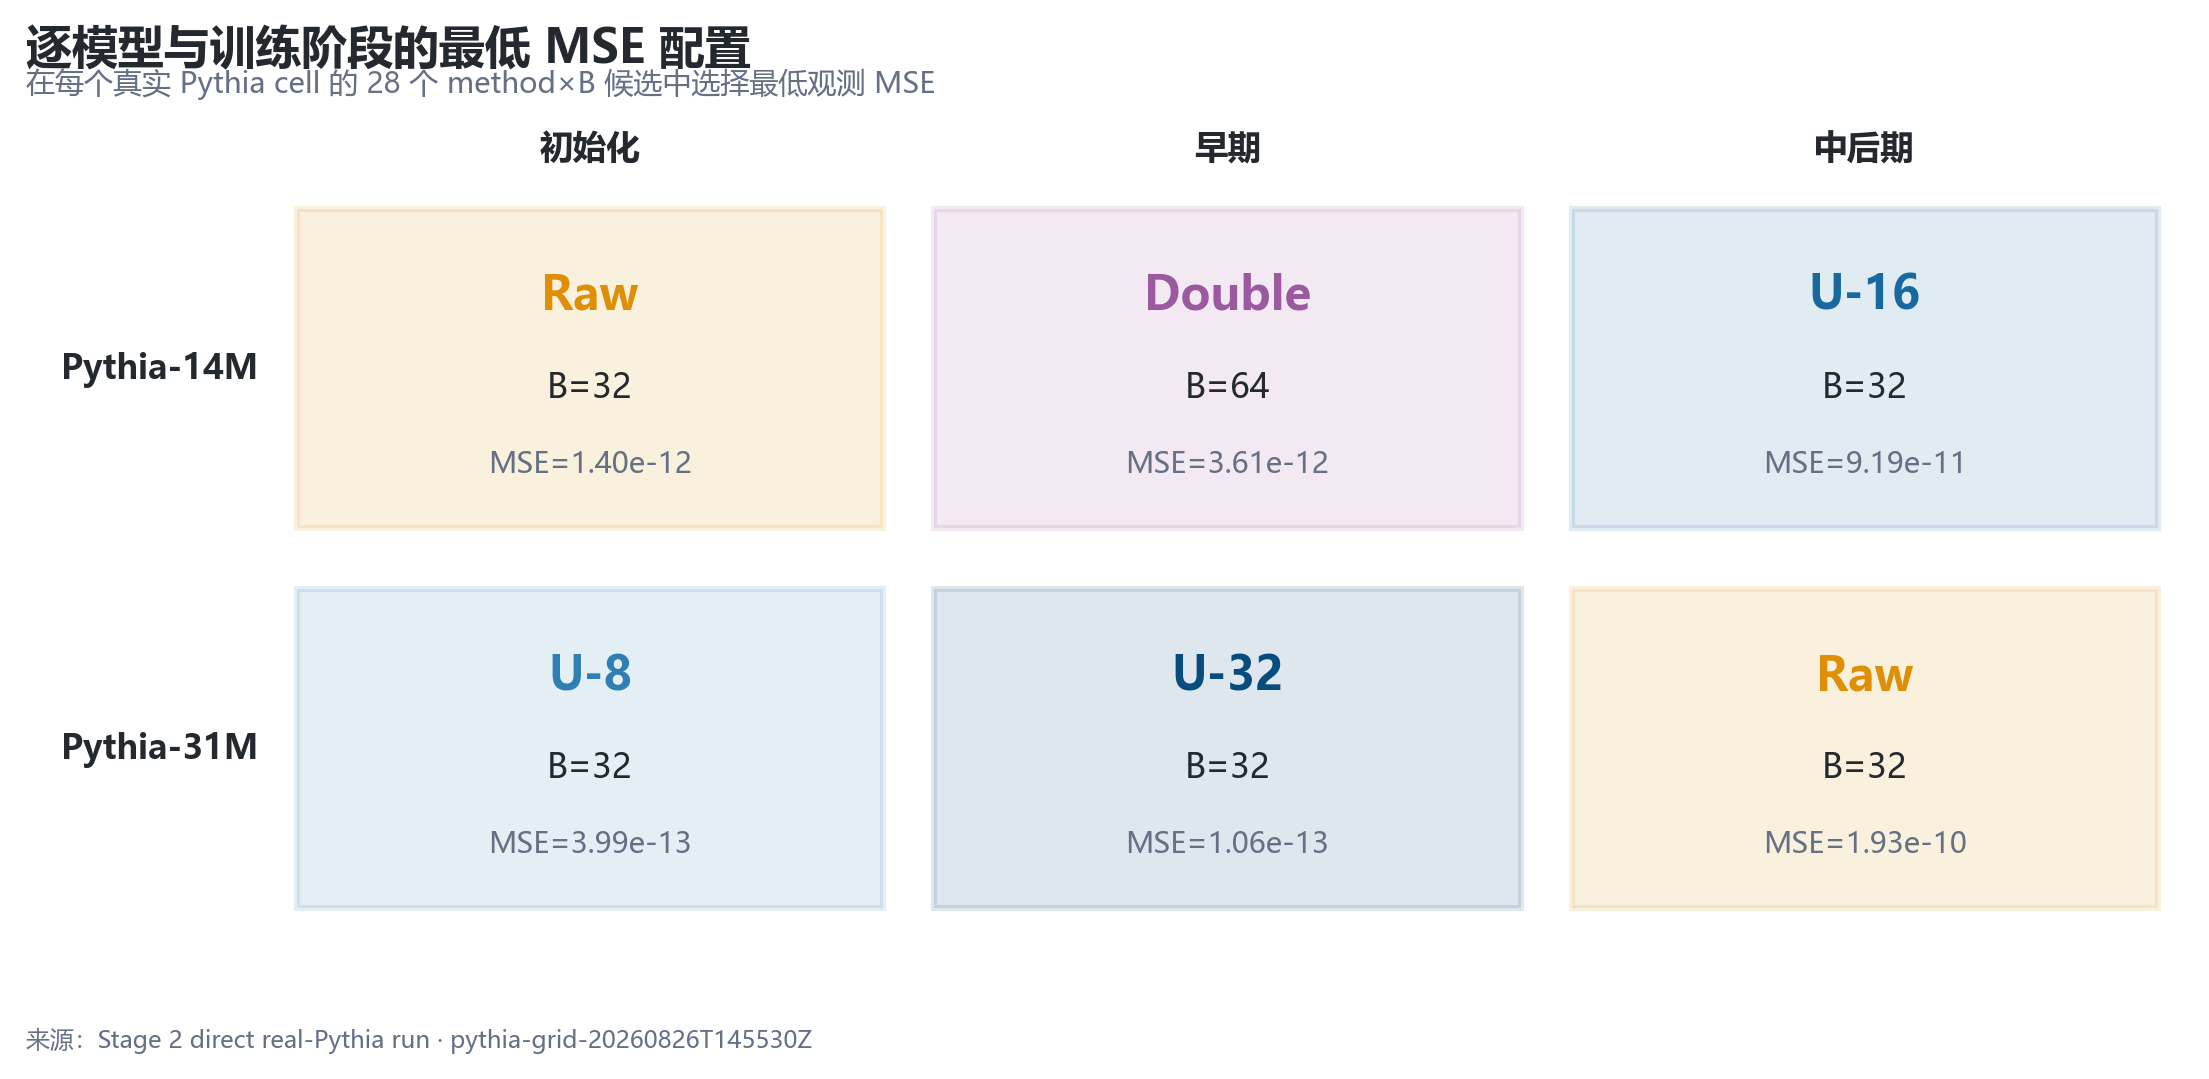
\includegraphics[width=0.98\textwidth]{fig02-cell-winners.png}
  \caption{六个真实 Pythia cell 的最低观测 MSE 配置。结果显示最优方法依赖模型规模与训练阶段。}
  \label{fig:cell-winners}
\end{figure}

\section{数据范围与分析口径}

\subsection{实验矩阵}

本次分析的基本单位是一个候选汇总
$(\text{model},\text{stage},B,\text{method})$。实验范围如下：

\begin{center}
\begin{tabularx}{0.94\textwidth}{>{\bfseries}lX}
  \toprule
  维度 & 取值 \\
  \midrule
  模型 & Pythia-14M（14,067,712 个坐标）；Pythia-31M-deduped（30,494,720 个坐标） \\
  阶段 & initialization、early、mid\_late \\
  样本预算 & $B\in\{32,64,128,256\}$ \\
  估计器 & Raw、Double、U-2、U-4、U-8、U-16、U-32 \\
  重复 & 通常每个 cell$\times B$ 为 64 次；一个续跑汇总为 18 次 \\
  候选数 & $2\times3\times4\times7=168$ \\
  \bottomrule
\end{tabularx}
\end{center}

\begin{figure}[H]
  \centering
  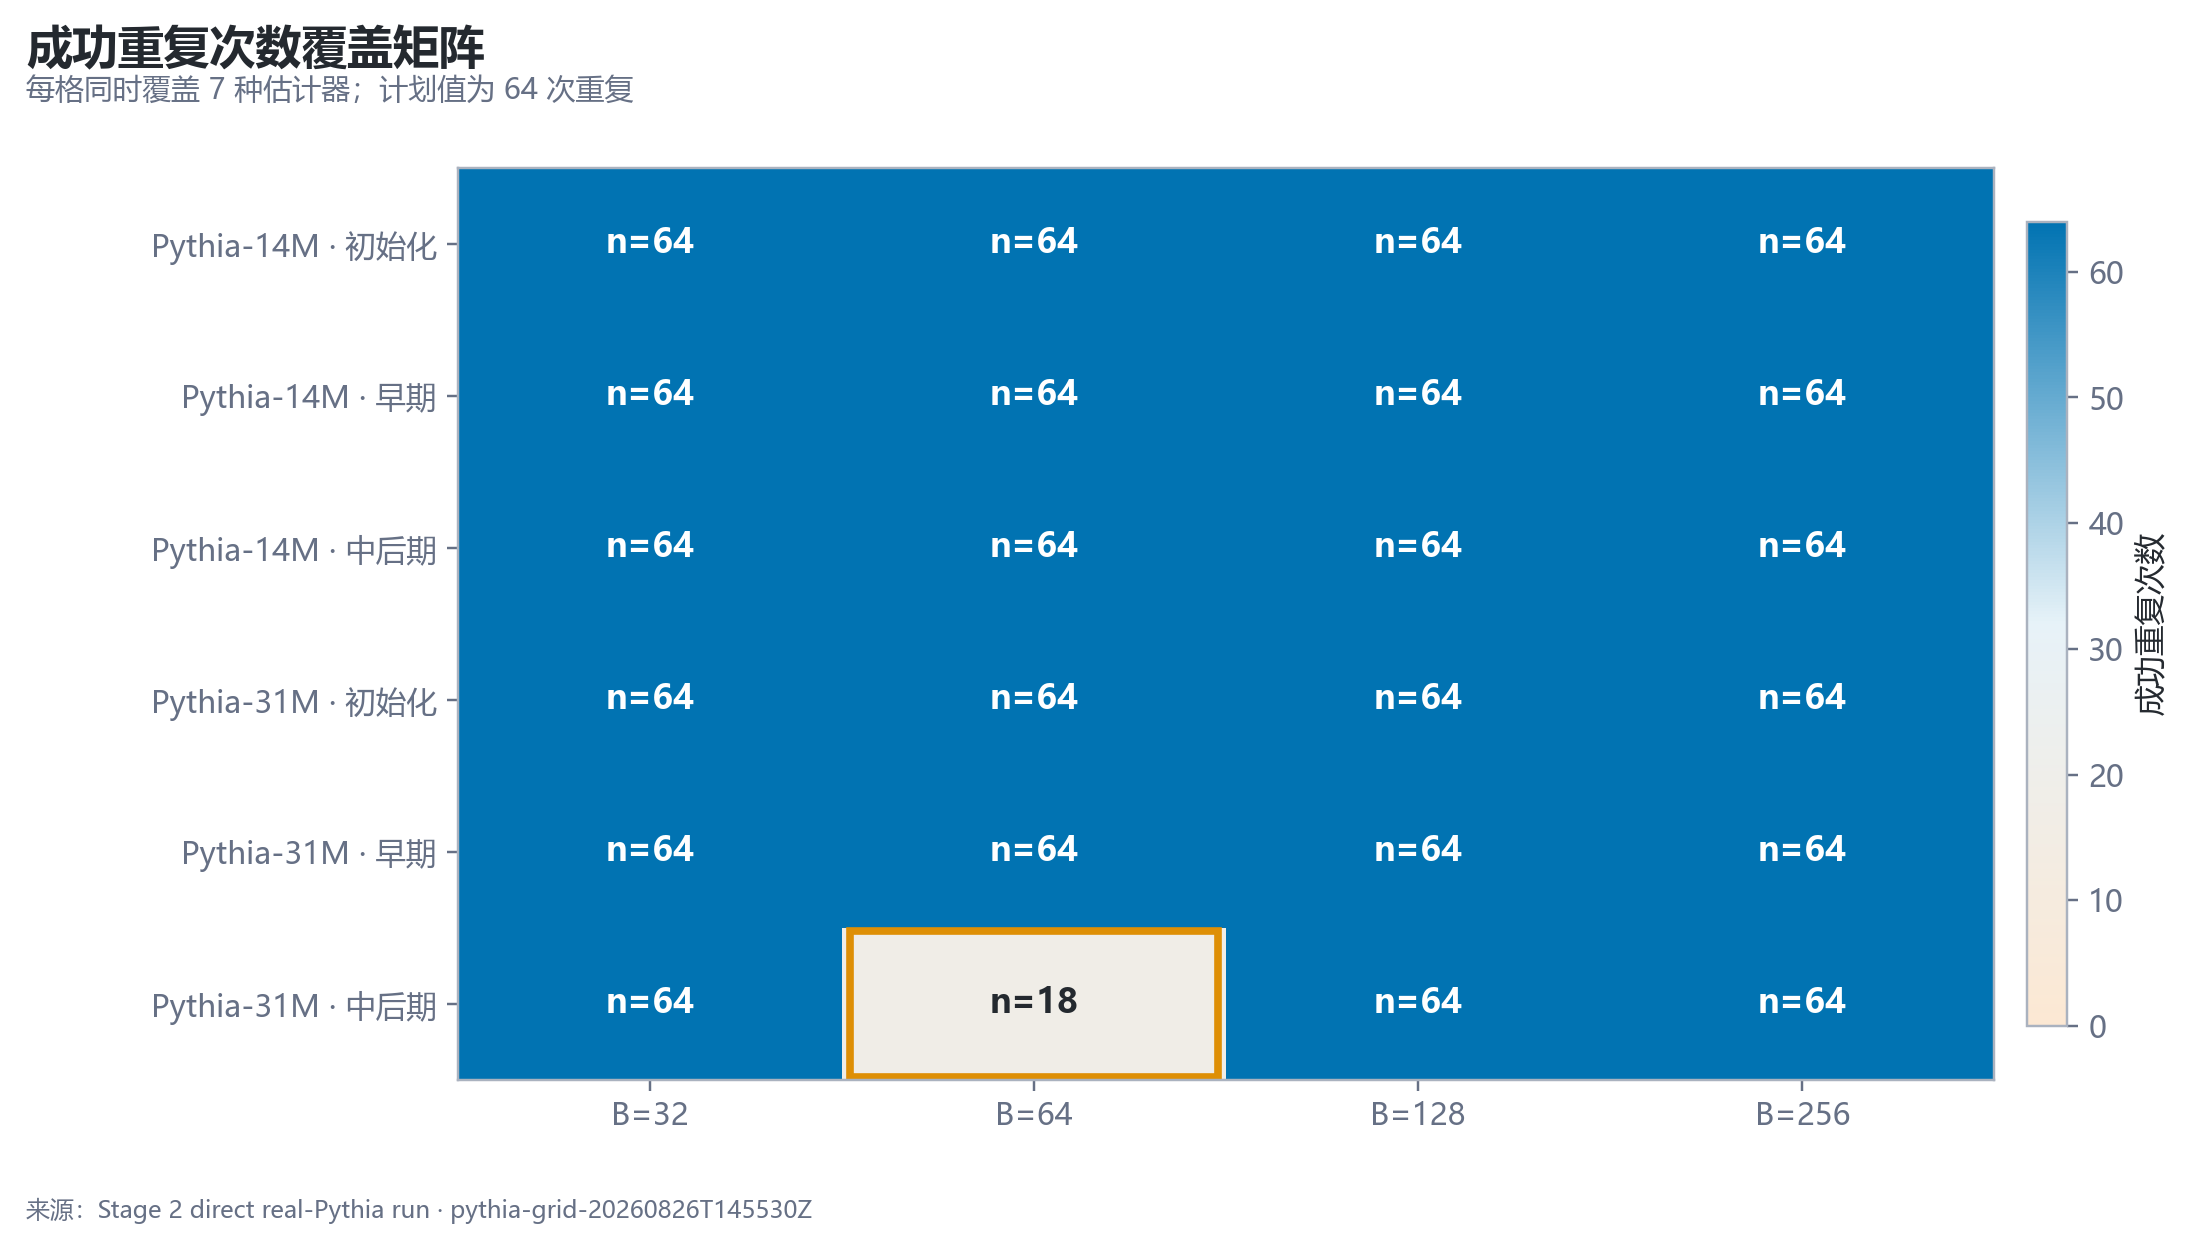
\includegraphics[width=0.96\textwidth]{fig01-coverage-matrix.png}
  \caption{进入精度比较的成功重复次数。每个格子的重复样本同时支持 7 种配对估计器。}
  \label{fig:coverage}
\end{figure}

Pythia-31M 中后期 $B=64$ 的原始运行在一个 CUDA 错误后由续跑段完成。
原始 JSONL 中保留了前段成功记录，但现有 Stage 2 交付的 7 个候选行均绑定
续跑段的 batch summary，因此图表使用该已发布汇总中的 $n=18$ 数值，不对
未保存完整坐标向量的两段均值进行事后近似合并。

\subsection{估计器定义}

设一个固定参数状态下的梯度统计单元为 $g_i$。Raw 估计器直接平方同一
样本池的平均梯度：
\begin{equation}
  \widehat I_{\mathrm{Raw}}
  =\left(\frac{1}{B}\sum_{i=1}^{B}g_i\right)^2.
\end{equation}
Double 将样本划分为两个互不重叠的半池：
\begin{equation}
  \widehat I_{\mathrm{Double}}=\bar g_A\,\bar g_B.
\end{equation}
U-$M$ 先形成 $M$ 个组梯度 $\tilde g_m$，再删除自乘项：
\begin{equation}
  \widehat I_{U,M}
  =\frac{\left(\sum_{m=1}^{M}\tilde g_m\right)^2
  -\sum_{m=1}^{M}\tilde g_m^2}{M(M-1)}.
\end{equation}
当 $M=2$ 时，U-2 与 Double 是同一代数构造。本次 168 行结果中，两者的
MSE、MAE 和 Pearson 最大绝对差分别为 $2.58\times10^{-26}$、0 和
$1.11\times10^{-16}$，属于浮点舍入量级。

\subsection{精度、排序与稳定性指标}

对于候选均值向量 $\widehat{\boldsymbol I}$ 与参考向量
$\boldsymbol I^{\star}$，报告使用：
\begin{align}
  \mathrm{MSE} &= \frac{1}{d}\sum_{k=1}^{d}
  (\widehat I_k-I_k^{\star})^2,\\
  \mathrm{MAE} &= \frac{1}{d}\sum_{k=1}^{d}
  |\widehat I_k-I_k^{\star}|,\\
  \rho &= \mathrm{Pearson}(\widehat{\boldsymbol I},\boldsymbol I^{\star}).
\end{align}
同时从 batch summary 中提取 signed bias mean，以及按坐标数加权的
between-repetition variance mean，用于描述偏差与重复稳定性。MSE/MAE
越低越好；Pearson 越接近 1，参数相对排序保持度越高。

\section{估计器比较结果}

\subsection{跨场景平均表现：U-32 最稳健，Raw 最分化}

图~\ref{fig:method-rank} 将每个 cell$\times B$ 内的 7 种方法按 MSE
排序，再对 24 个场景取平均。排名指标避免不同模型和阶段的 MSE 绝对尺度
直接相加。\method{U-32} 的平均排名最低；\method{U-16} 与 \method{U-8}
紧随其后。三者的跨场景几何平均 MSE 仅相差 0.017\% 以内，因此
\method{U-32} 的优势主要是\emph{跨场景排序更稳定}，而不是数量级差异。

\begin{figure}[H]
  \centering
  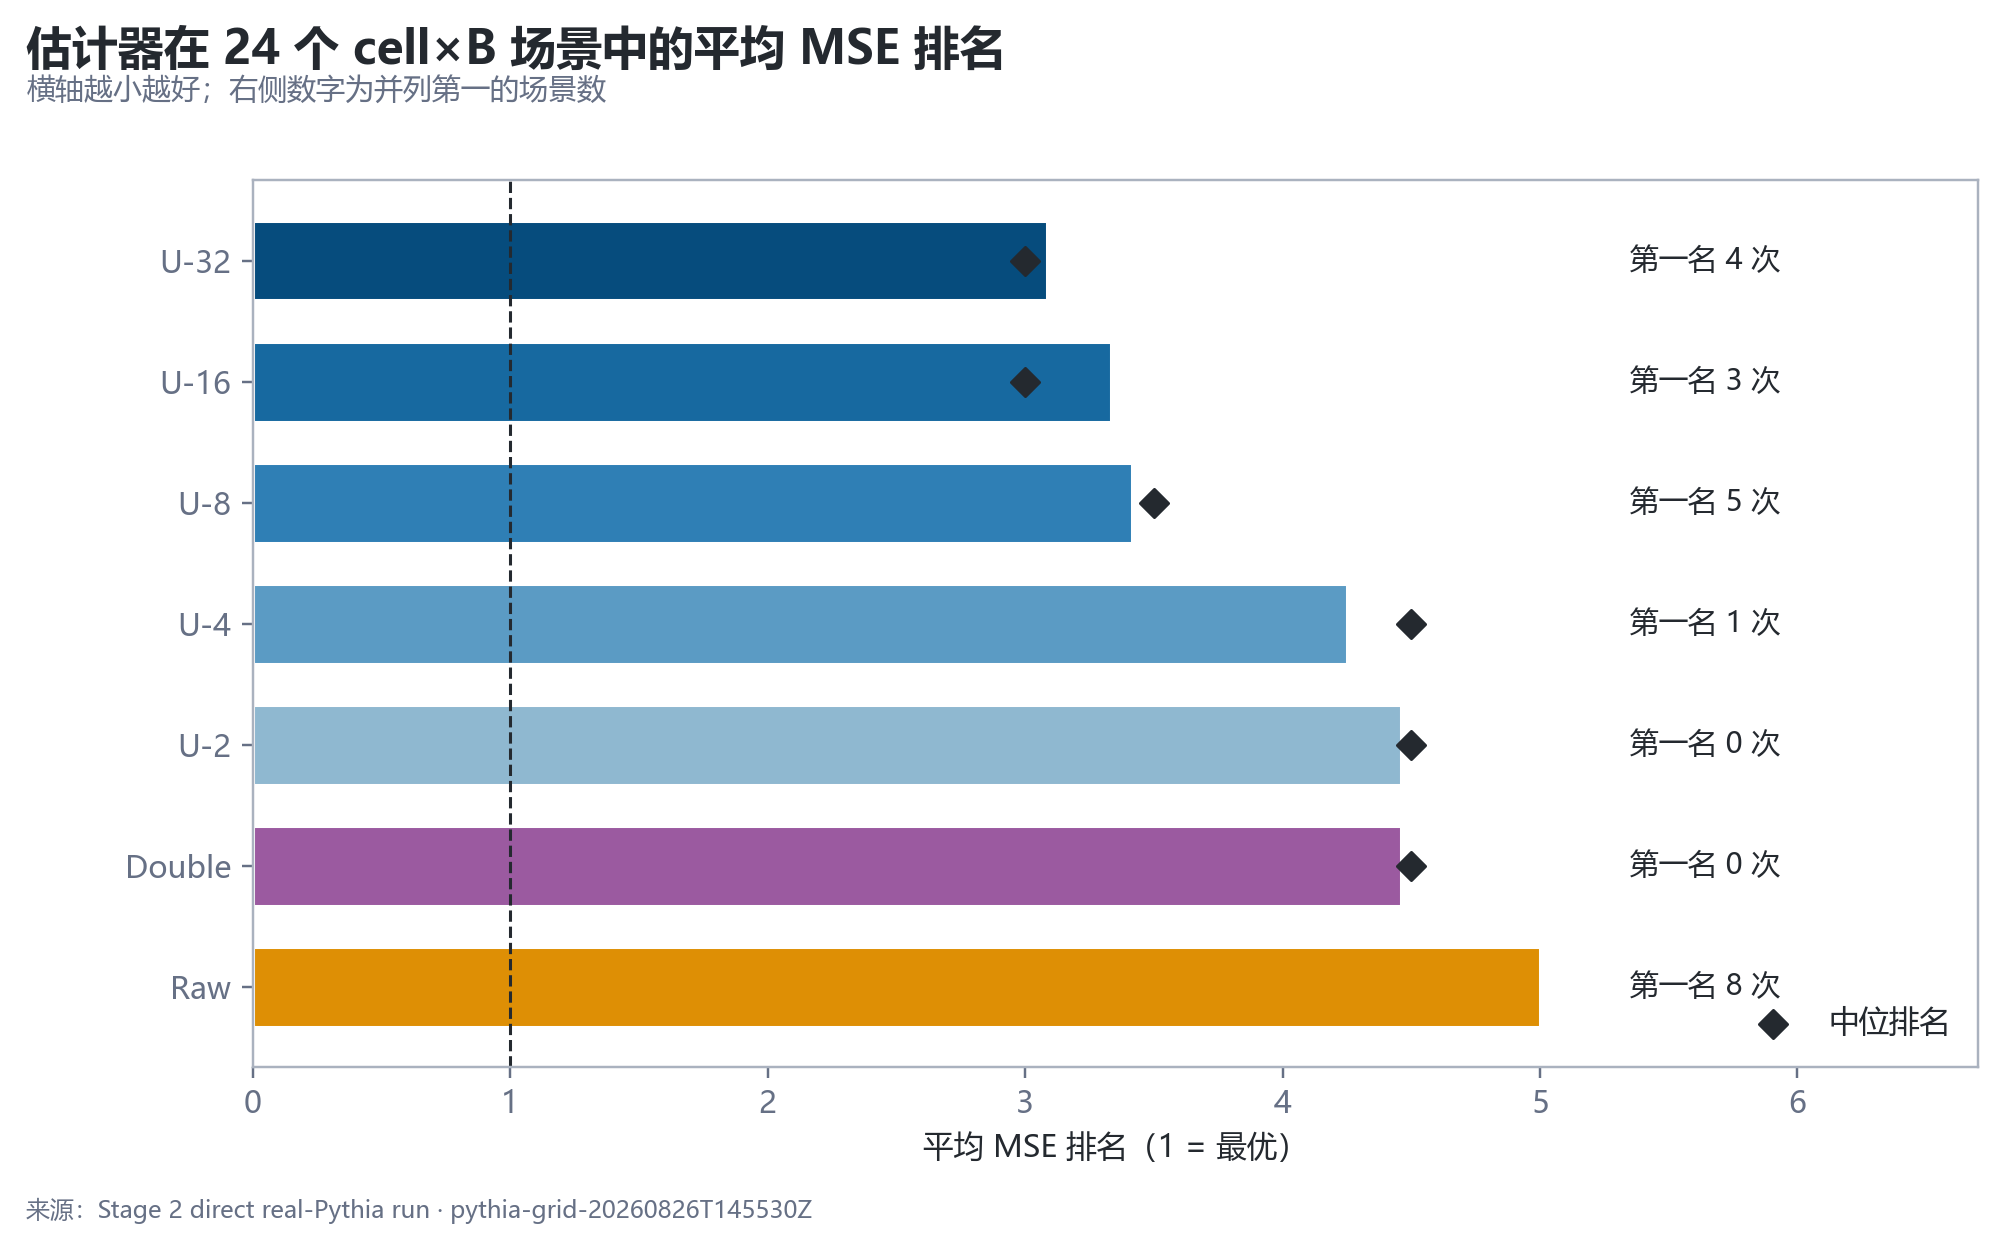
\includegraphics[width=0.97\textwidth]{fig03-method-rank.png}
  \caption{24 个 cell$\times B$ 场景的平均 MSE 排名。菱形为中位排名；Double 与 U-2 的排名完全一致。}
  \label{fig:method-rank}
\end{figure}

\begin{center}
\begin{tabular}{lrrrr}
  \toprule
  方法 & 平均排名 & 第一名次数 & 几何平均 MSE/Raw & Pearson 中位数 \\
  \midrule
  \textbf{U-32} & \textbf{3.08} & 4 & \textbf{0.9241} & \textbf{0.9252} \\
  U-16 & 3.33 & 3 & 0.9242 & 0.9252 \\
  U-8  & 3.42 & 5 & 0.9243 & 0.9250 \\
  U-4  & 4.25 & 1 & 0.9252 & 0.9238 \\
  Double & 4.46 & 0 & 0.9269 & 0.9237 \\
  U-2    & 4.46 & 0 & 0.9269 & 0.9237 \\
  Raw    & 5.00 & \textbf{8} & 1.0000 & 0.9182 \\
  \bottomrule
\end{tabular}
\end{center}

\method{Raw} 的 8 次第一名与中位第 7 名同时存在，说明它不是稳定地
“第二梯队”，而是随 cell 改变在最好与最差之间切换。这一模式决定了
后续实验应保留 Raw 作为对照，却不应仅凭少数逐 cell 胜出结果将其设为
统一默认。

\begin{figure}[H]
  \centering
  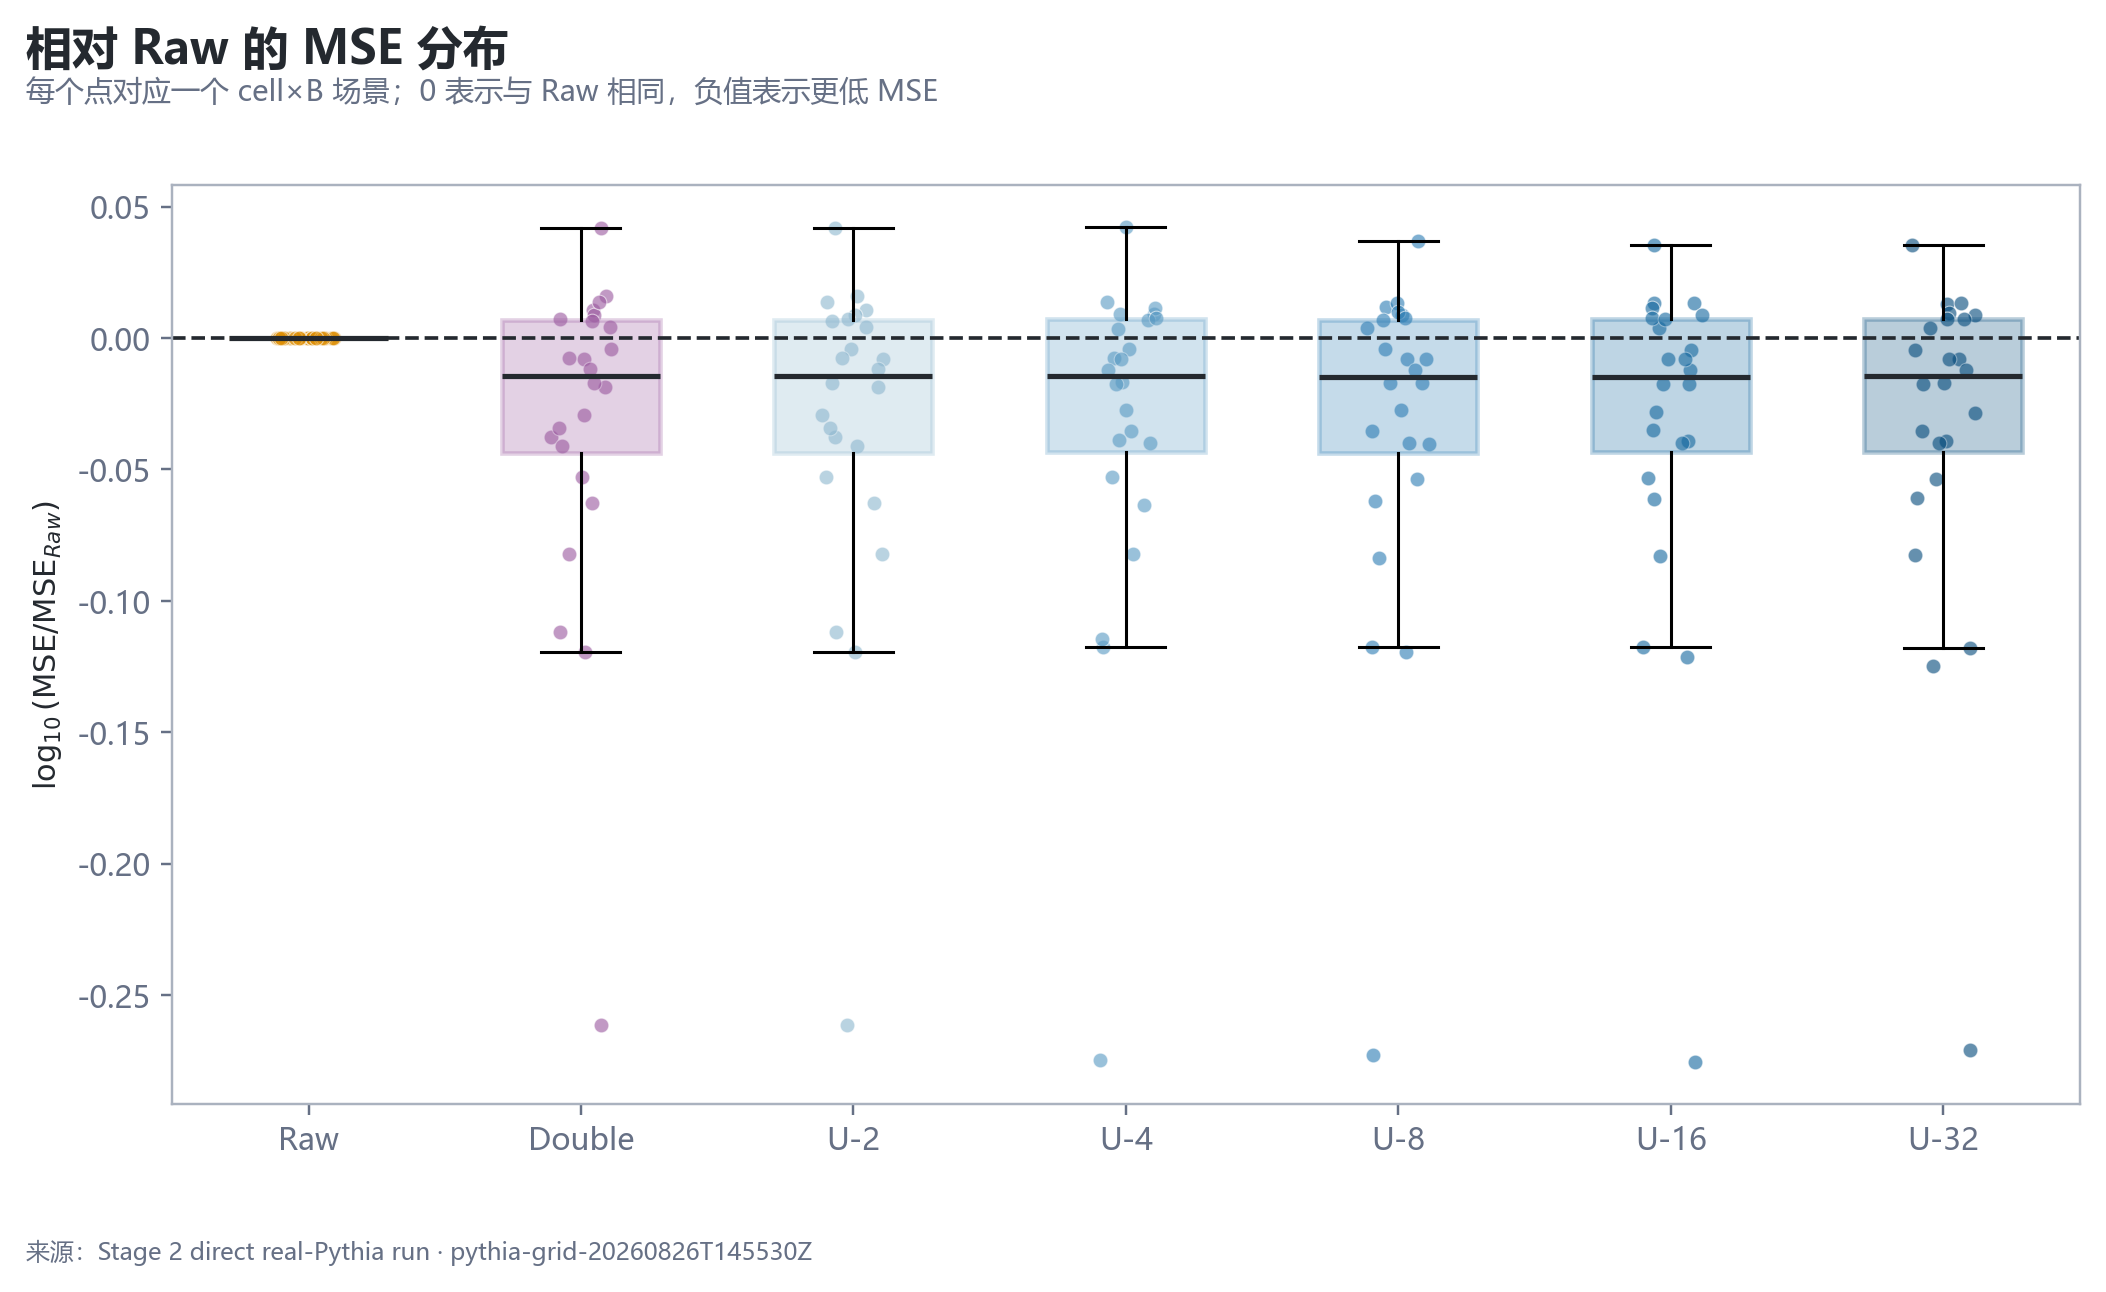
\includegraphics[width=0.97\textwidth]{fig04-relative-mse.png}
  \caption{各方法相对同一 cell$\times B$ 下 Raw 的 MSE。U 系列和 Double 的中位数均低于 Raw，但分布包含场景反转。}
  \label{fig:relative-mse}
\end{figure}

\subsection{模型与阶段依赖}

Pythia-14M 与 Pythia-31M 的完整曲线分别见图~\ref{fig:mse14} 和
图~\ref{fig:mse31}。U 系列曲线在多数位置紧密重合，Raw 则经常与
无偏化方法分离。分阶段汇总显示：

\begin{itemize}
  \item \textbf{初始化：}U-8 的平均排名最好（3.25），但 Raw 在两个模型的
    8 个 batch 场景中有 4 次第一；应采用 U-8 主分析加 Raw 敏感性对照。
  \item \textbf{早期：}U-32 平均排名 2.25，Raw 在 8 个场景中平均排名第 7；
    这是 U-32 最明确的适用阶段。
  \item \textbf{中后期：}U-16 与 U-32 平均排名同为 3.625；Raw 在两个模型上
    呈现不同方向，因此建议 U-16/U-32 主分析并保留 Raw。
\end{itemize}

\begin{figure}[p]
  \centering
  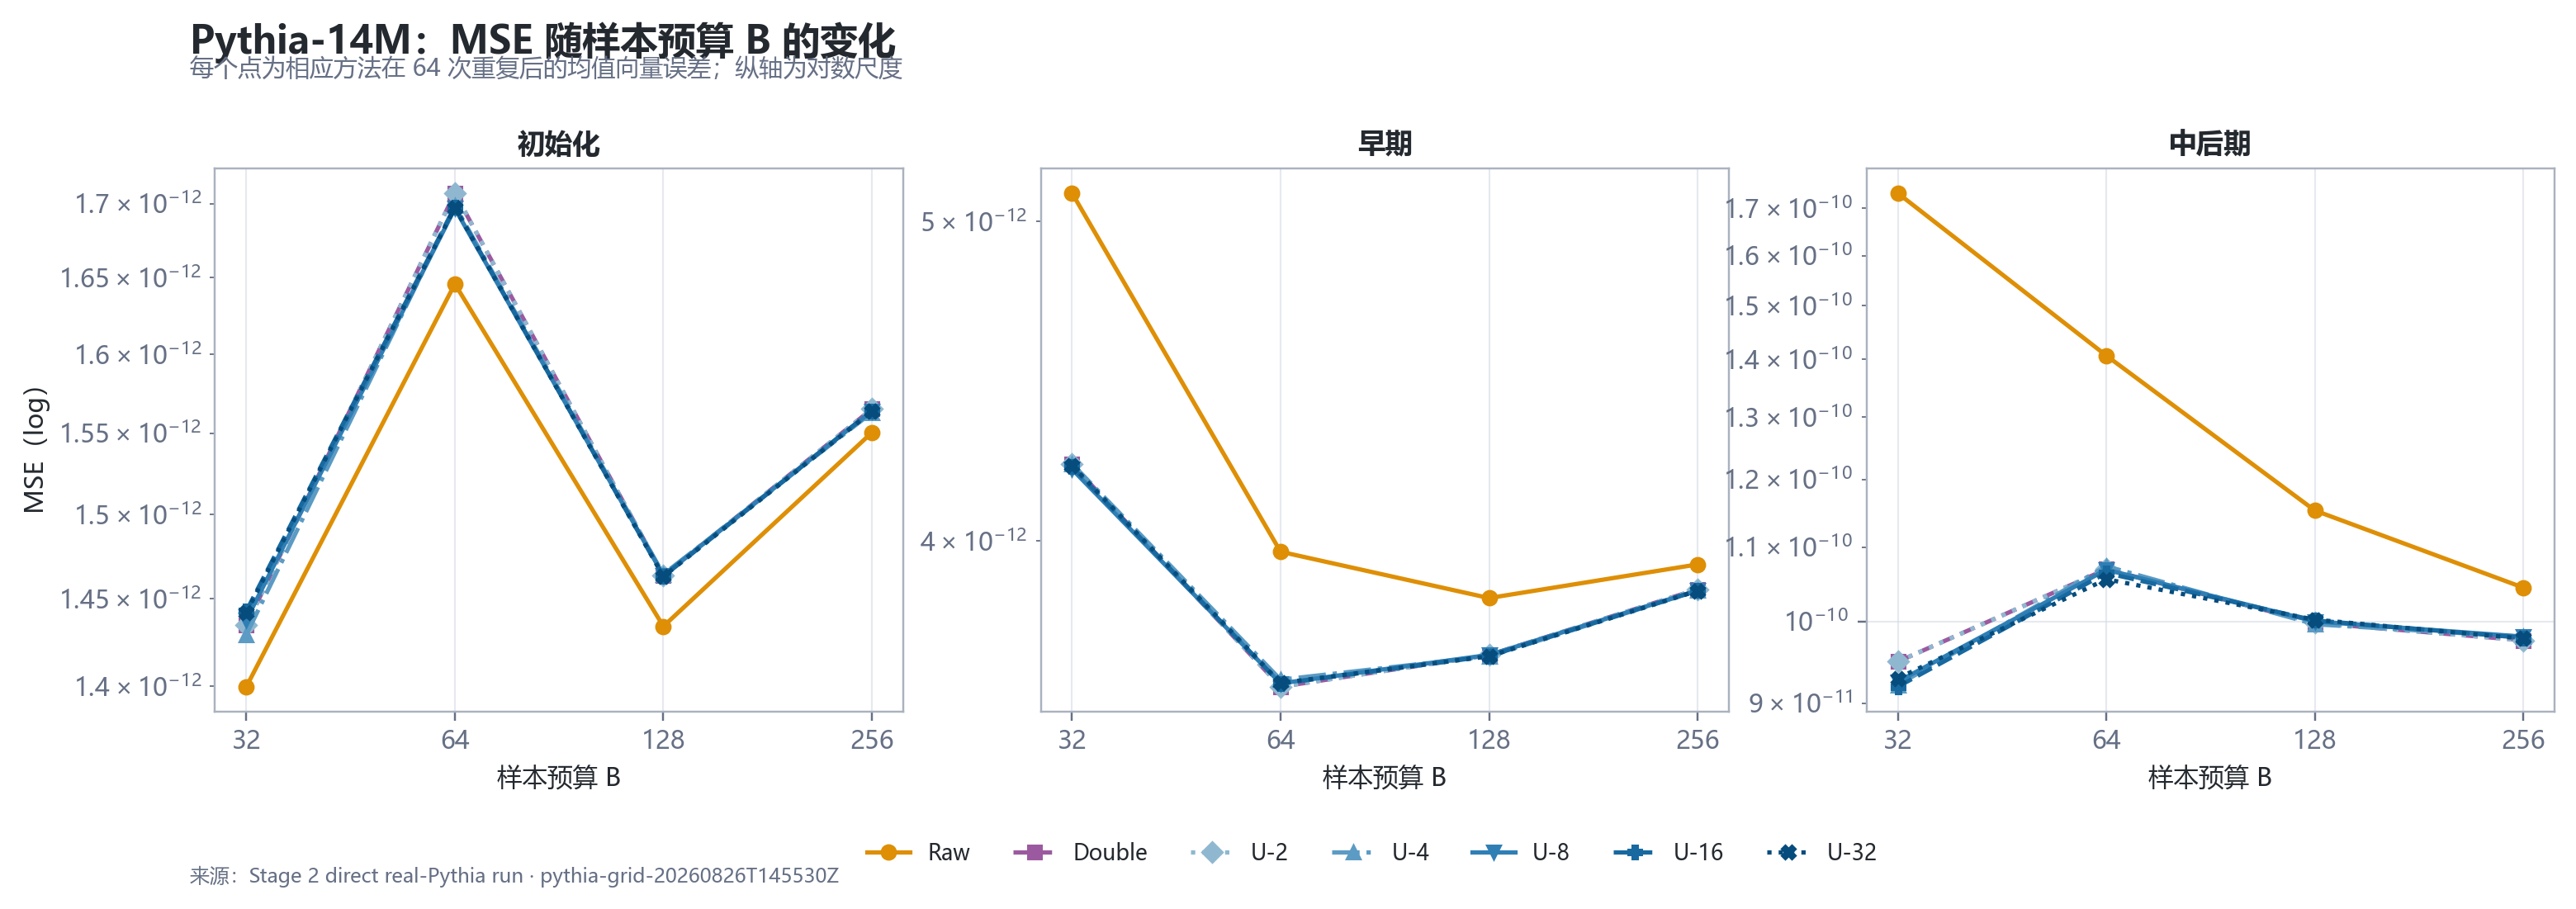
\includegraphics[width=\textwidth]{fig05-mse-by-batch-14m.png}
  \caption{Pythia-14M 中不同估计器的 MSE--$B$ 曲线。Double 与 U-2 曲线重合。}
  \label{fig:mse14}
\end{figure}

\begin{figure}[p]
  \centering
  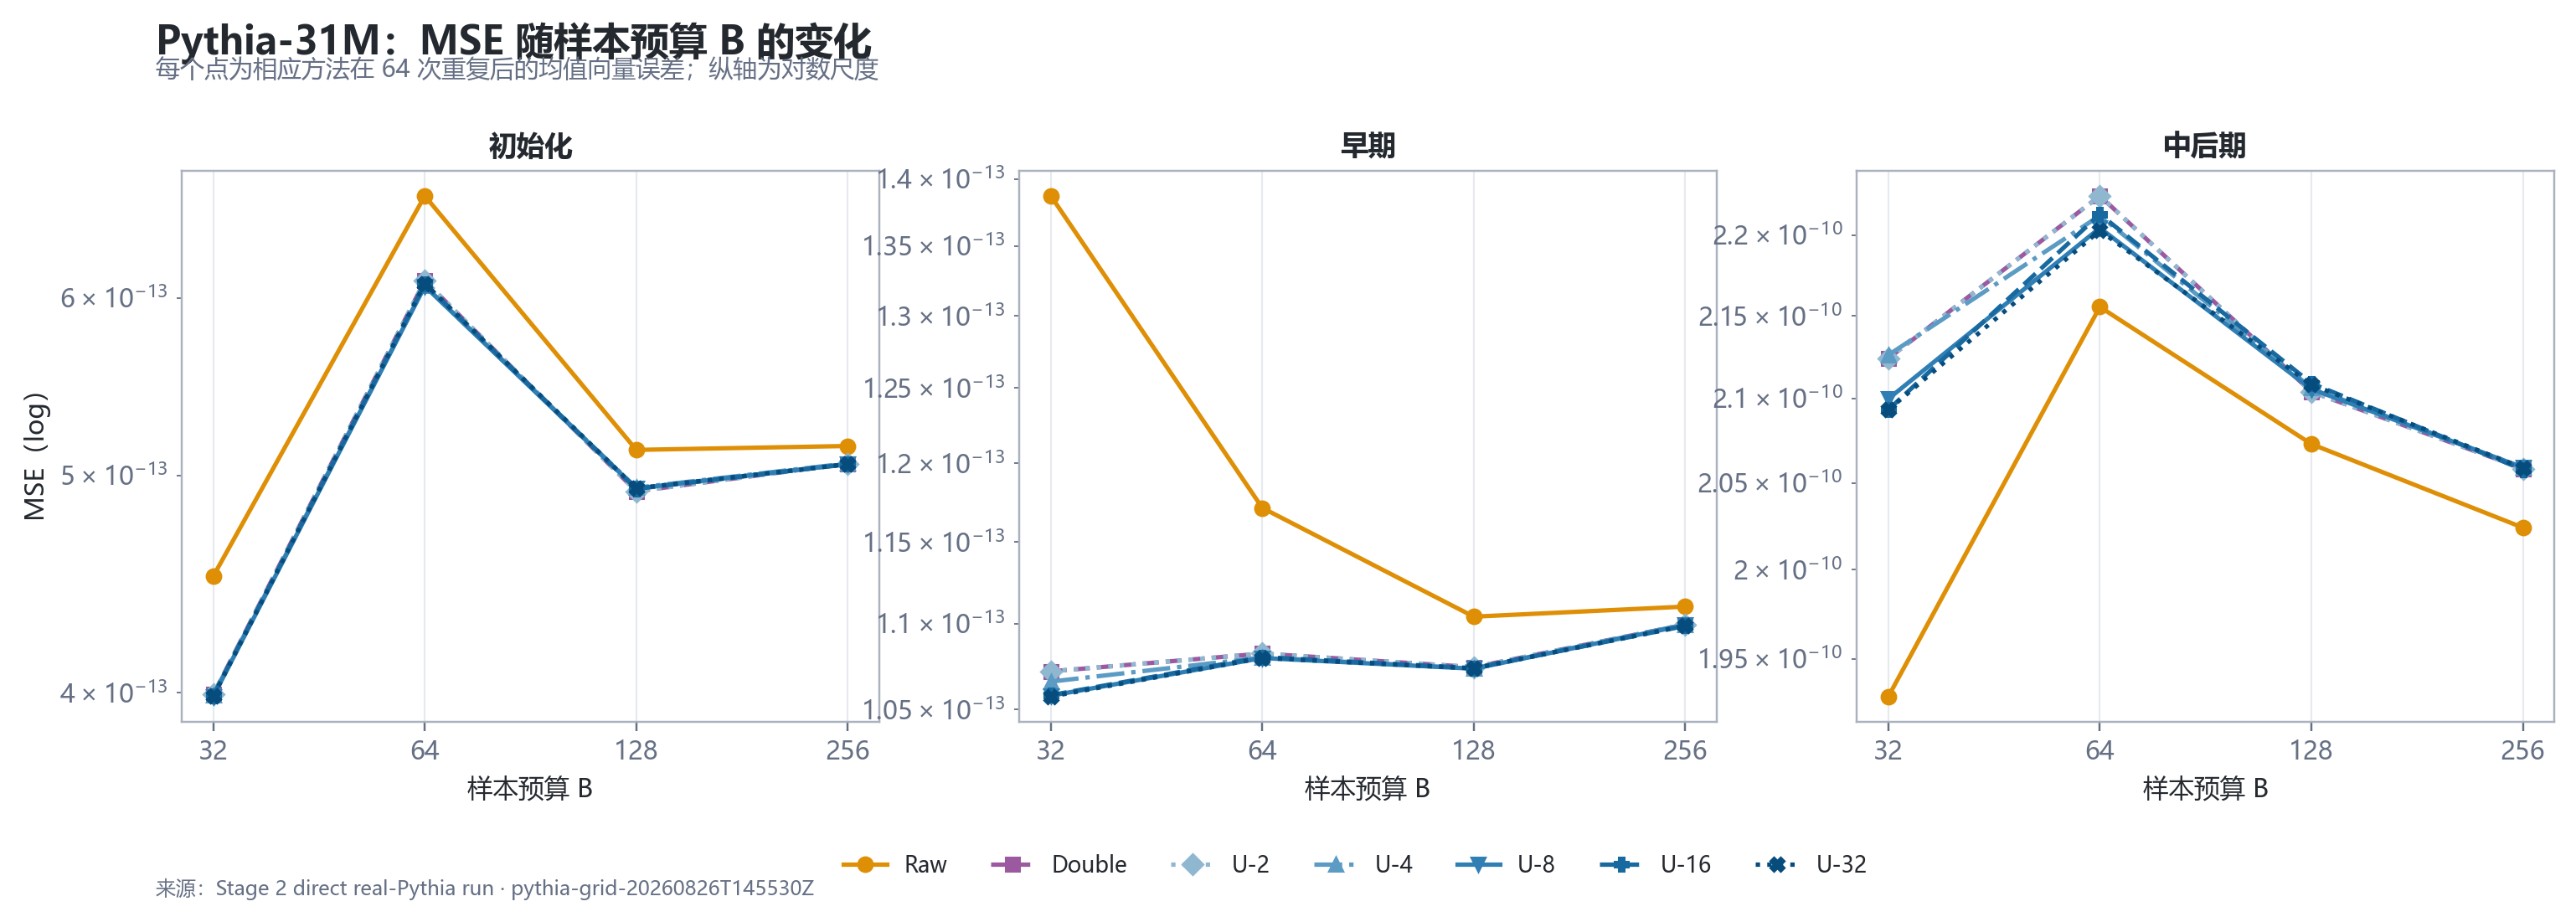
\includegraphics[width=\textwidth]{fig06-mse-by-batch-31m.png}
  \caption{Pythia-31M 中不同估计器的 MSE--$B$ 曲线。中后期 $B=64$ 点使用已交付的 $n=18$ 续跑汇总。}
  \label{fig:mse31}
\end{figure}

\FloatBarrier

\subsection{排序保持度与偏差--方差位置}

Pearson 指标的跨方法差异小于 MSE 排名差异。U-32 的 Pearson 中位数为
0.92523，Raw 为 0.91821。换言之，无偏化方法对全坐标误差的改善更明显，
而全局排序保持度的改善较温和。

\begin{figure}[H]
  \centering
  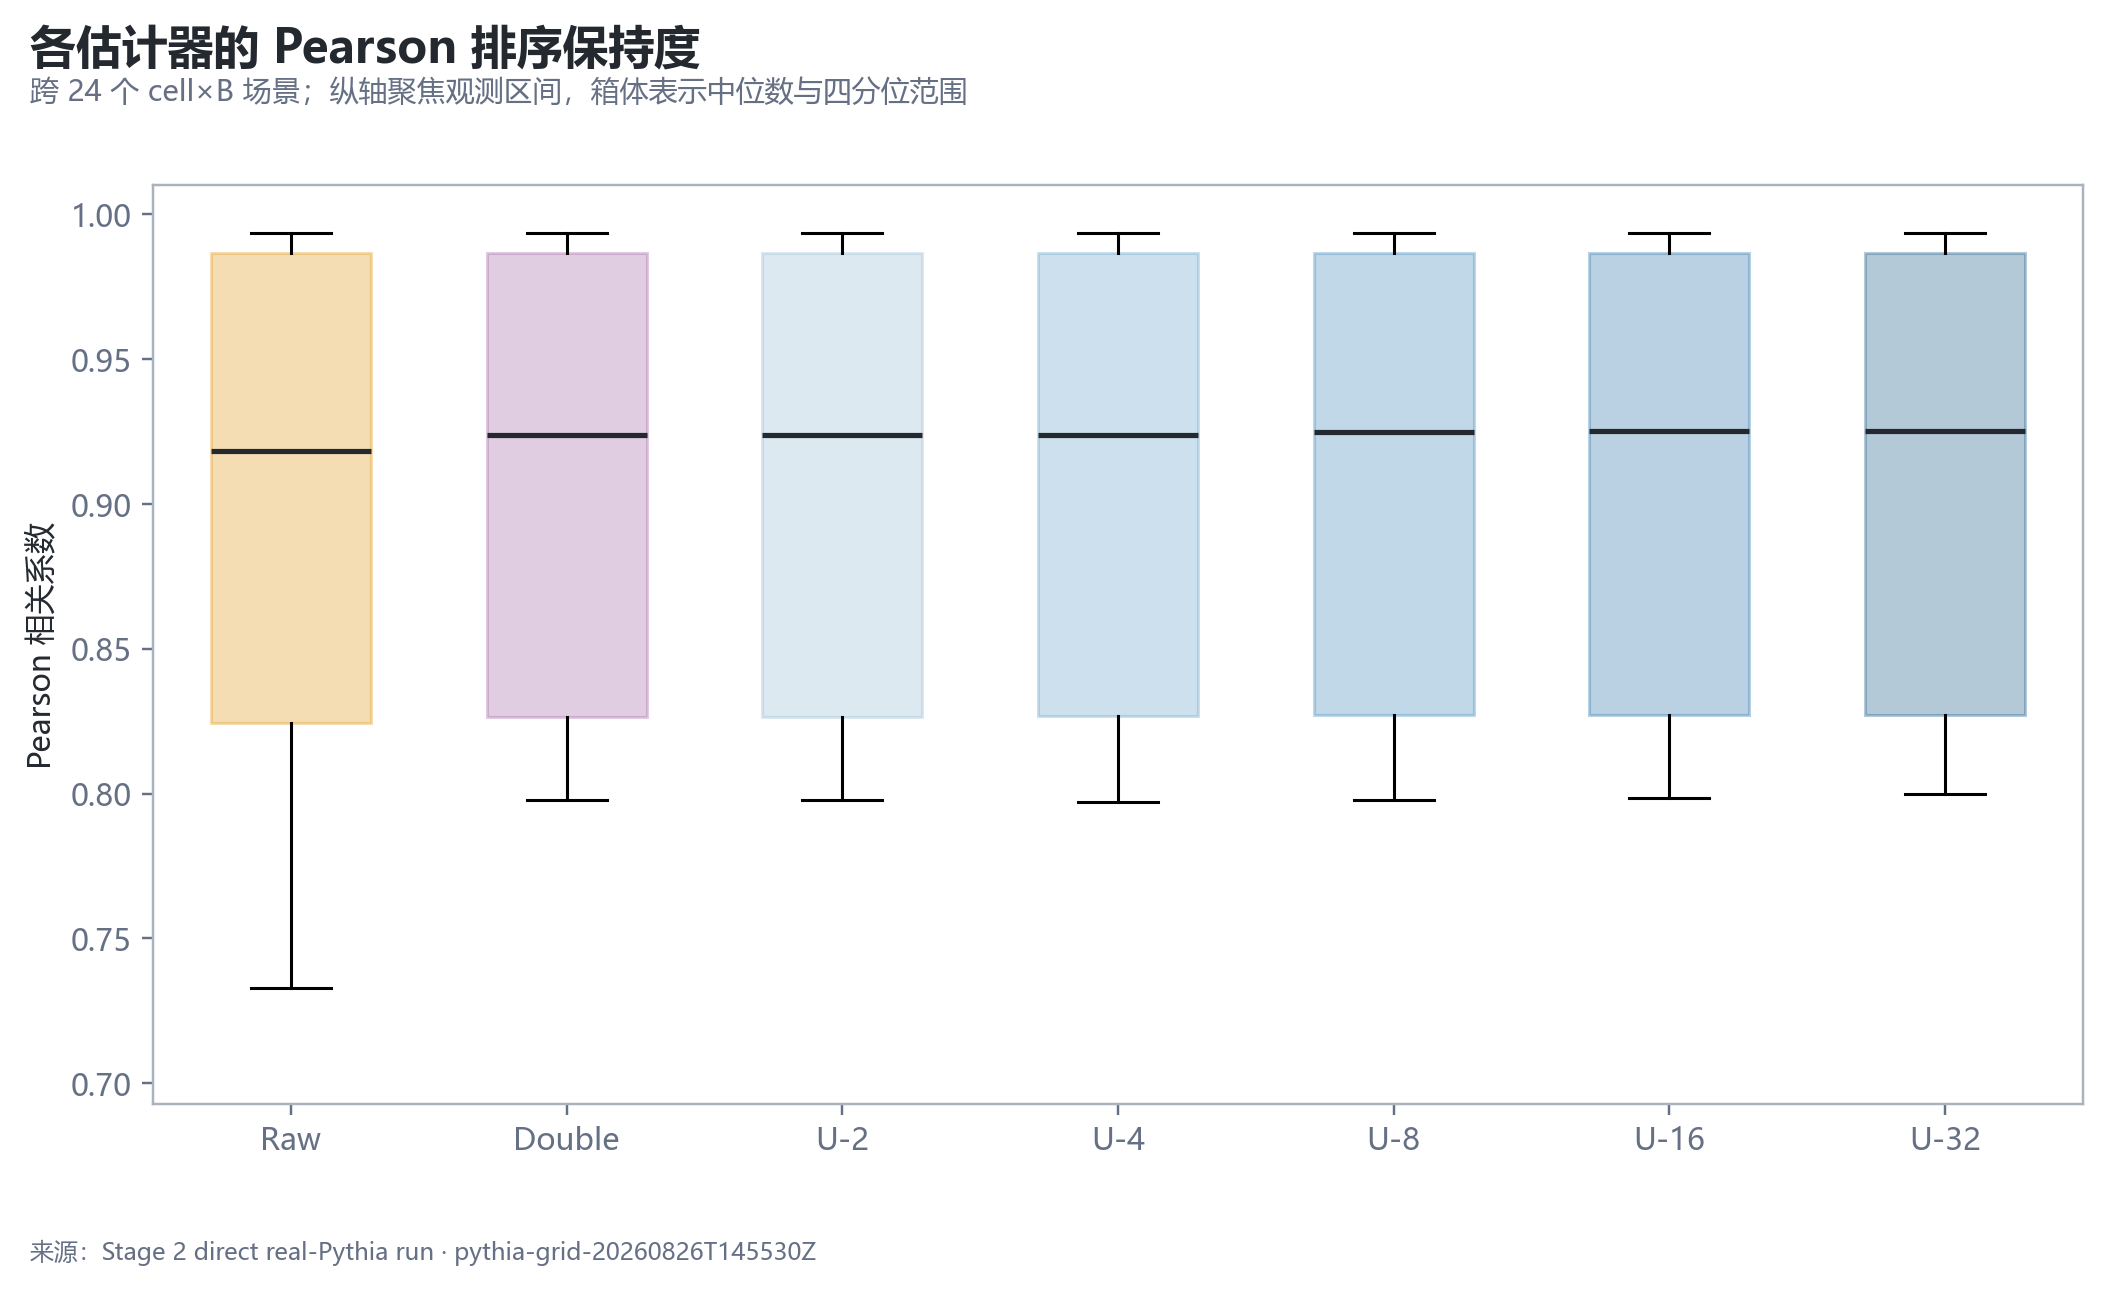
\includegraphics[width=0.96\textwidth]{fig07-pearson-distribution.png}
  \caption{24 个场景中 Pearson 相关系数的分布。纵轴聚焦观测区间。}
  \label{fig:pearson}
\end{figure}

U-32 相对 Raw 的 signed bias 绝对值中位数降低 28.17\%，逐坐标跨重复
方差中位数降低 2.56\%。U-8、U-16 与 U-32 聚集在相近区域，再次说明
U 系列内部差异较小；最重要的结构性差异是 Raw 与无偏化方法之间的分离。

\begin{figure}[H]
  \centering
  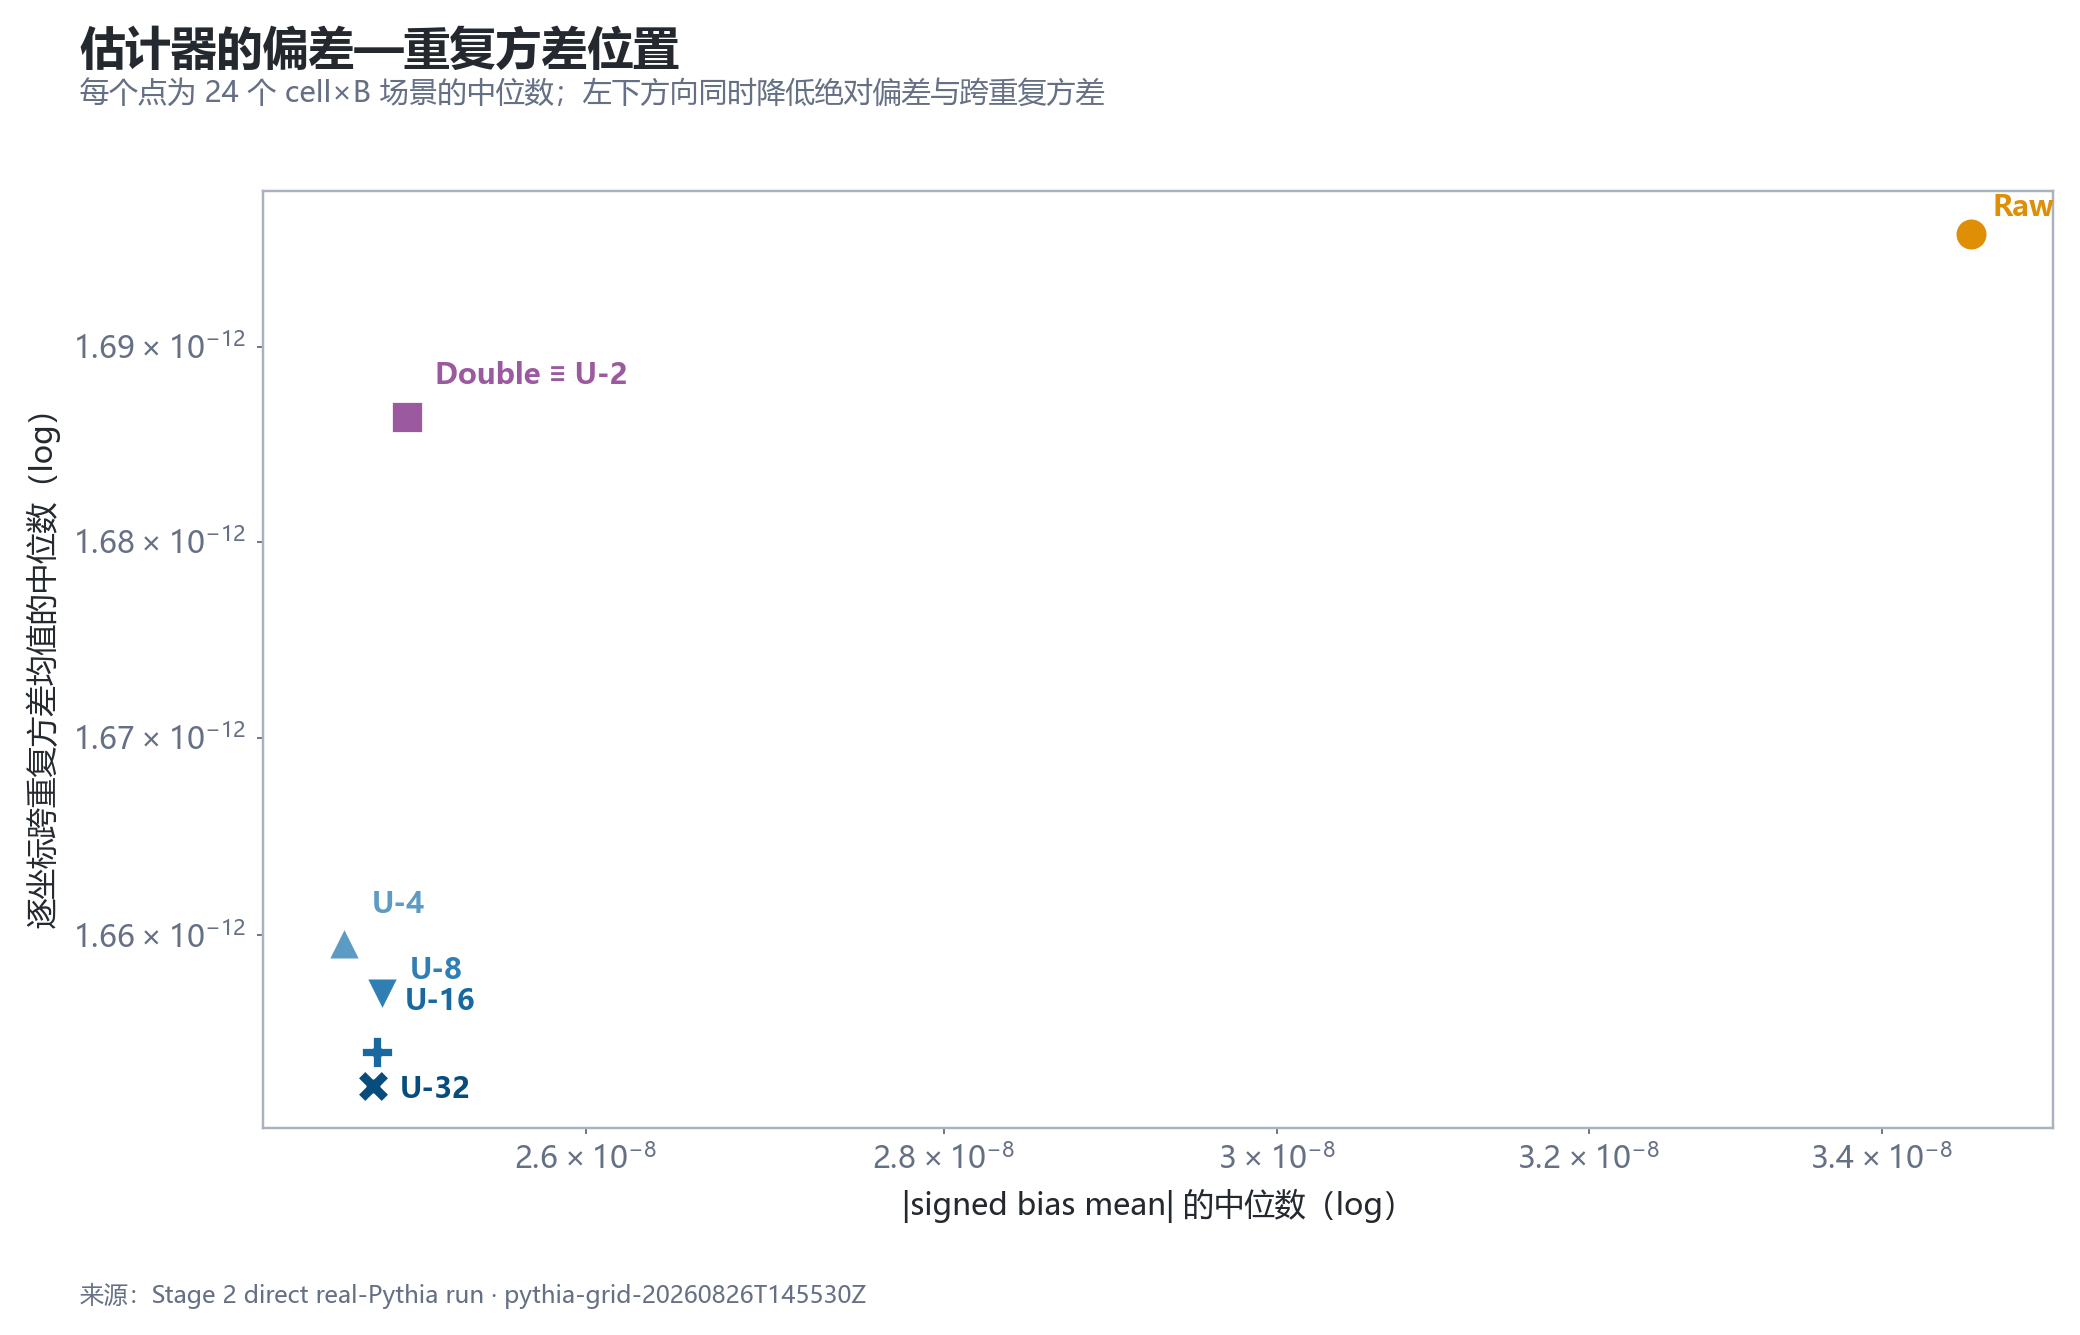
\includegraphics[width=0.92\textwidth]{fig08-bias-variance.png}
  \caption{偏差--重复方差位置。Double 与 U-2 完全重合；左下方表示两项指标同时较低。}
  \label{fig:bias-variance}
\end{figure}

\section{样本预算、时间与显存}

\subsection{\texorpdfstring{$B=32$}{B=32} 在当前比较中最常取得最低 MSE}

对每个 cell$\times$method 单独选择最低 MSE 的 $B$，$B=32$ 在 42 个
比较中胜出 27 次（64.3\%）。$B=128$ 仅胜出 2 次。该结果意味着当前
任务中更大样本预算并未单调改善相对参考向量的误差，因此后续实验不应
默认把更大 $B$ 当作更高精度配置。

\begin{figure}[H]
  \centering
  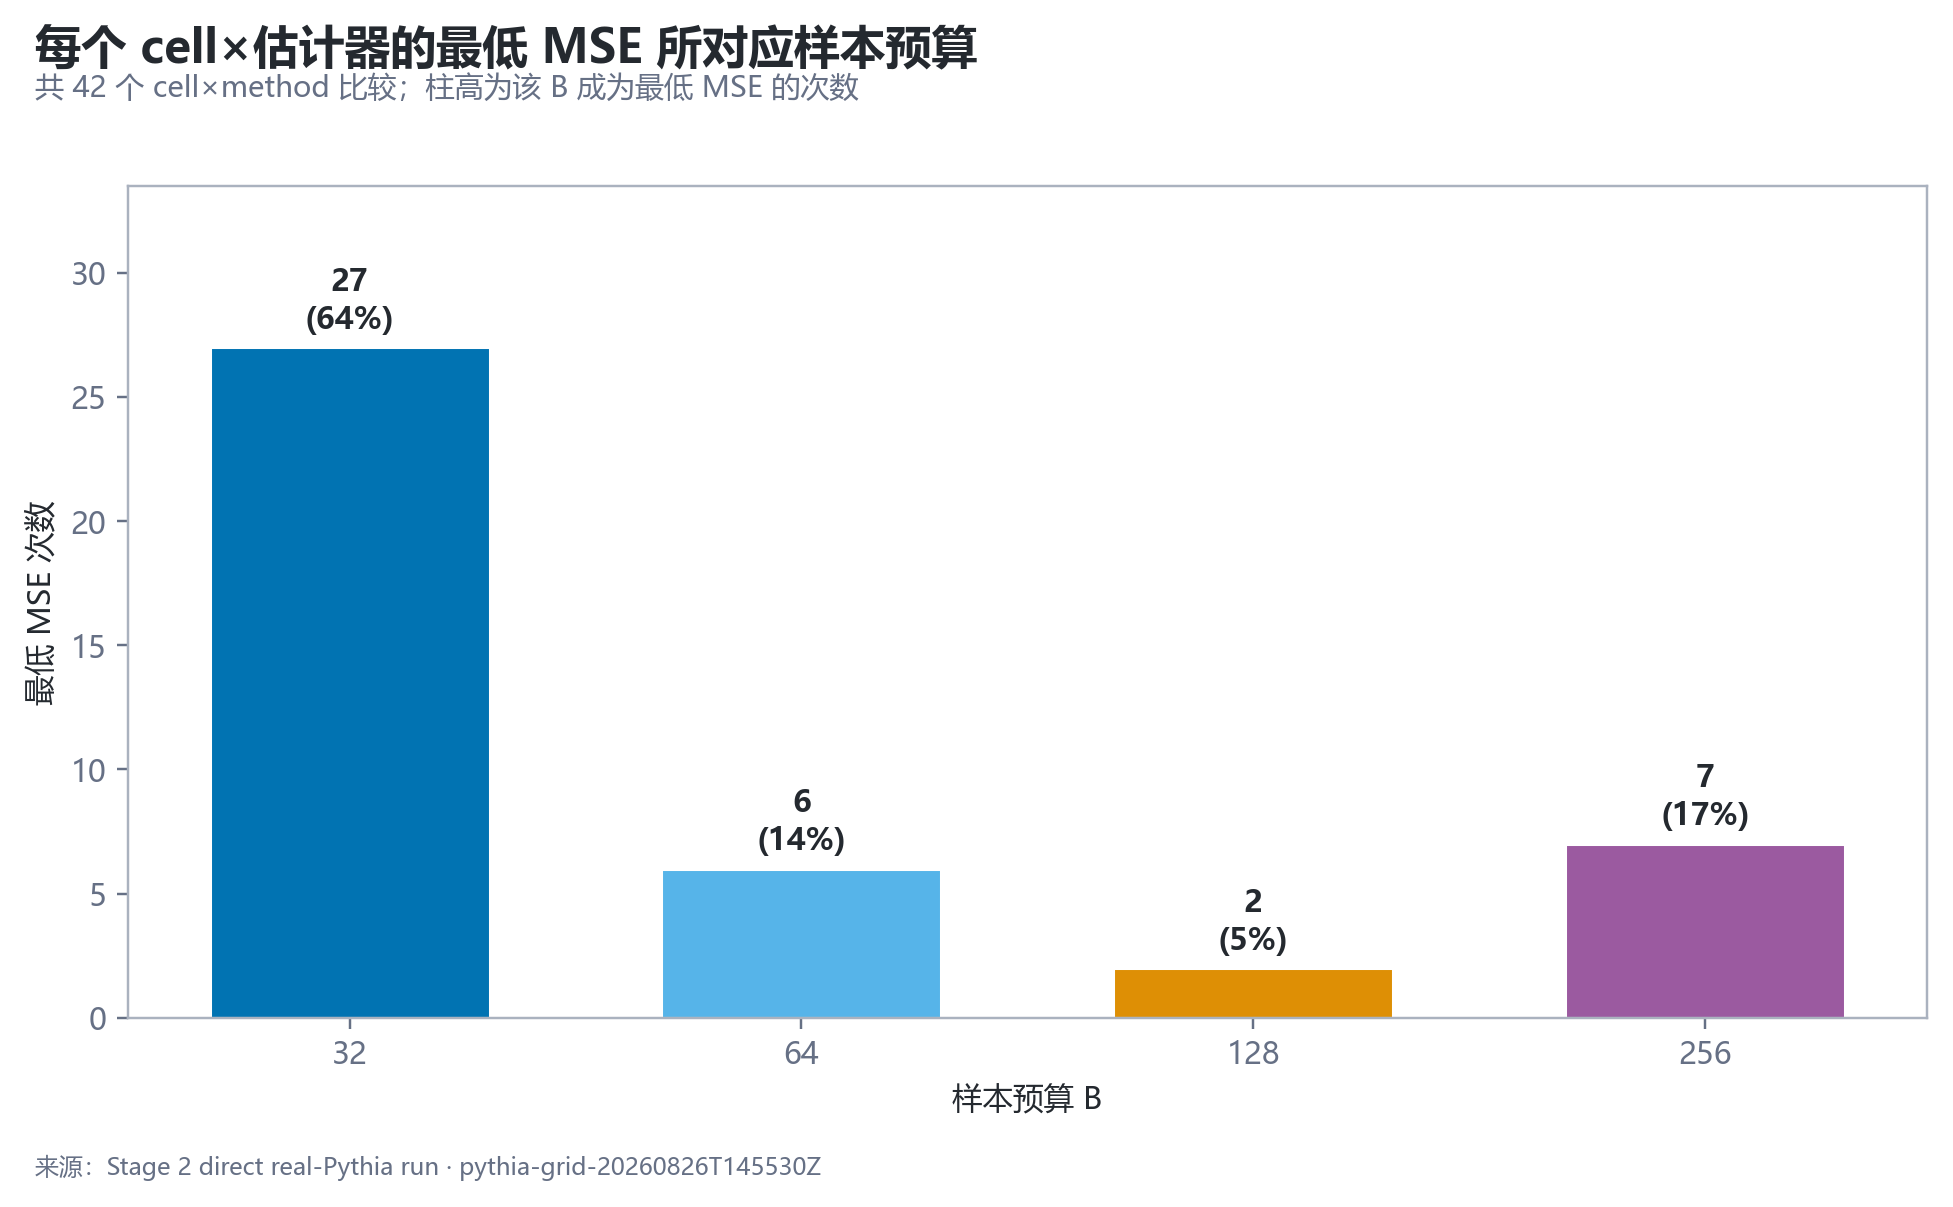
\includegraphics[width=0.90\textwidth]{fig09-best-batch-frequency.png}
  \caption{42 个 cell$\times$method 比较中，各样本预算取得最低 MSE 的次数。}
  \label{fig:batch-frequency}
\end{figure}

\subsection{时间随 \texorpdfstring{$B$}{B} 上升，显存主要由模型规模决定}

每次 repetition 同时计算 Raw、Double 与全部 U-$M$，所以 profiler
不能拆出单个估计器的独立耗时。它能回答的是：在同一套估计器输出下，
样本预算 $B$ 的总体成本如何变化。六个 cell 的中位壁钟时间从 $B=32$
的 7.71 秒增长到 $B=256$ 的 12.65 秒，即 1.64 倍。峰值显存则在同一
模型内基本稳定，Pythia-14M 约 11.9--12.1 GiB，Pythia-31M 约
25.7--26.1 GiB。

\begin{figure}[p]
  \centering
  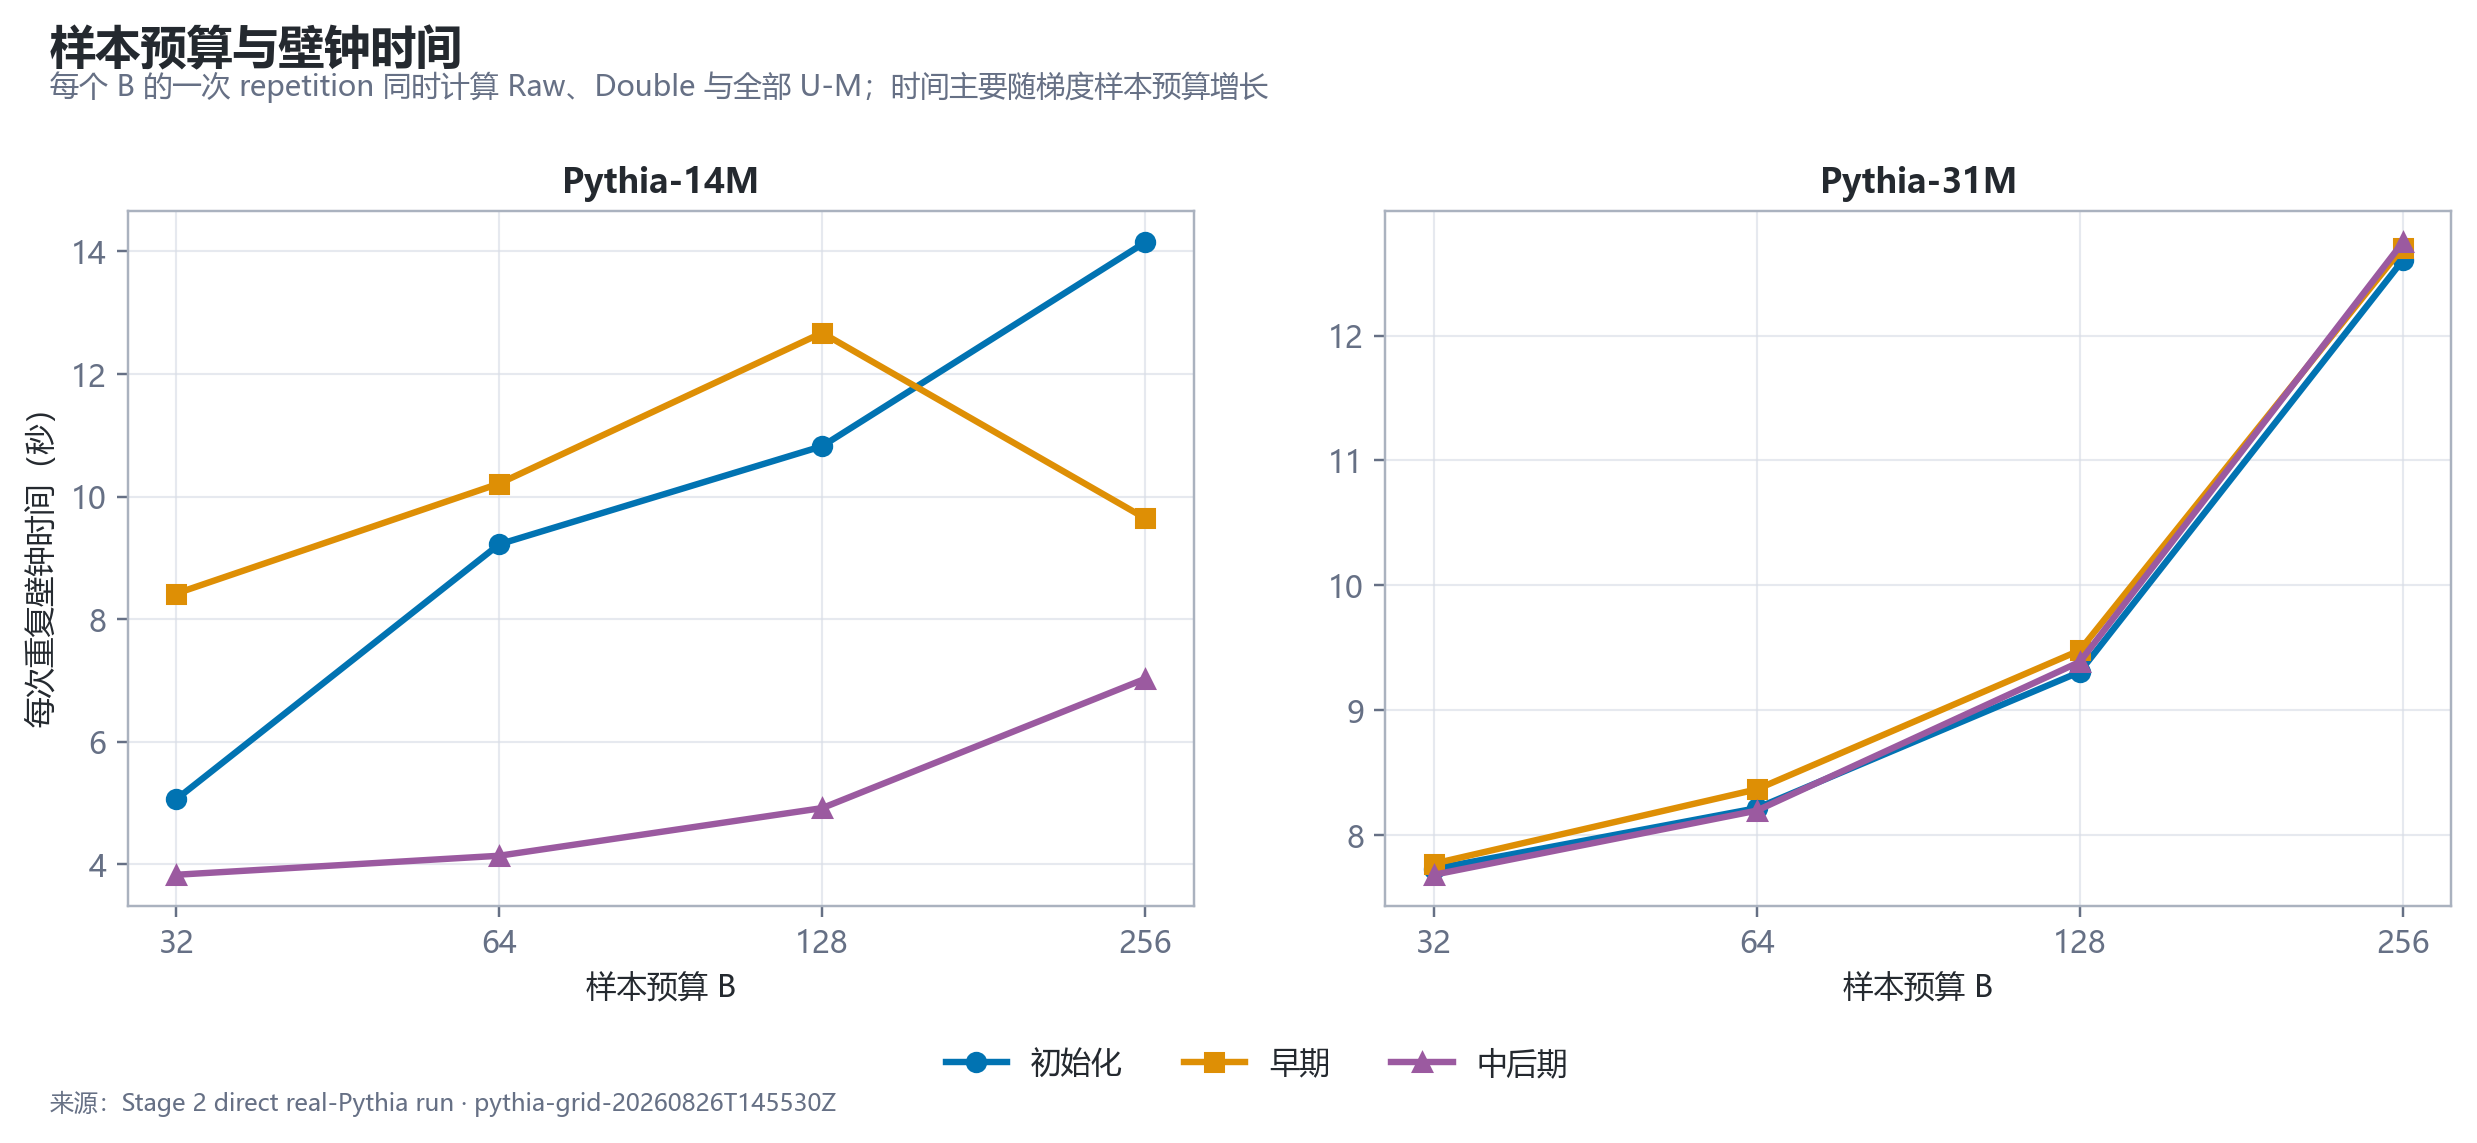
\includegraphics[width=\textwidth]{fig10-runtime-scaling.png}
  \caption{样本预算与每次重复壁钟时间。Pythia-14M early 的非单调点说明共享运行环境中存在计时波动。}
  \label{fig:runtime}
\end{figure}

\begin{figure}[p]
  \centering
  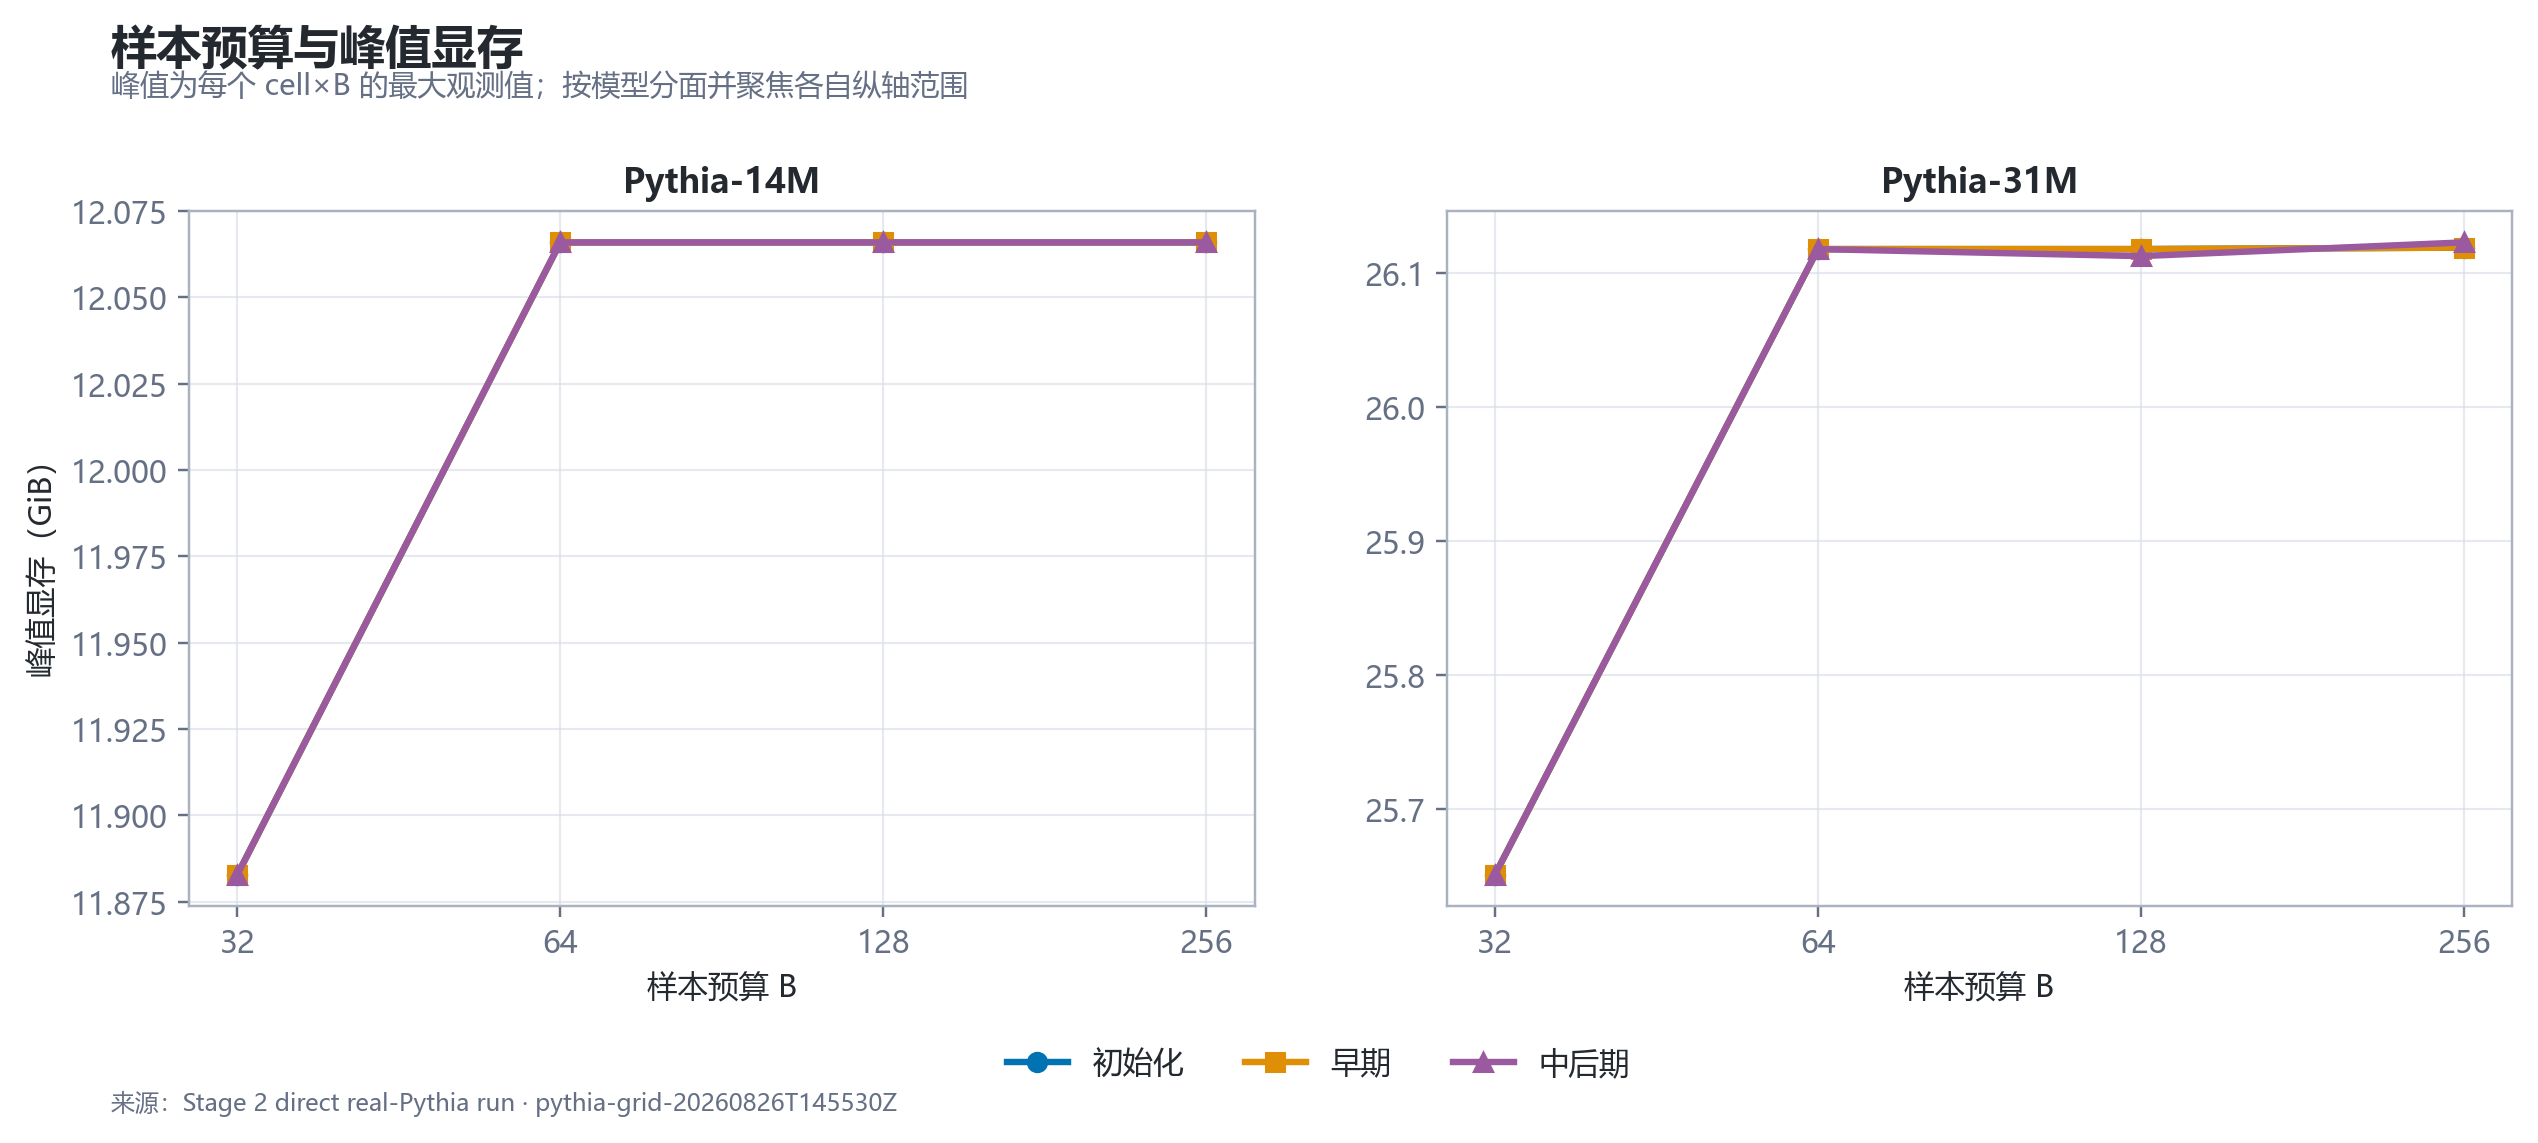
\includegraphics[width=\textwidth]{fig11-memory-scaling.png}
  \caption{样本预算与峰值显存。纵轴按模型分别聚焦局部范围。}
  \label{fig:memory}
\end{figure}

\FloatBarrier

\subsection{精度--时间联合选择}

图~\ref{fig:pareto} 在每个 cell、每个 $B$ 中只保留最低 MSE 方法。
五个 cell 的全局最低 MSE 位于 $B=32$；Pythia-14M early 的例外是
\method{Double}、$B=64$。因此，\key{$B=32$ 是统一运行的默认点}，
而 \method{Double}、$B=64$ 是一个明确但窄的 early-stage 特化点。

\begin{figure}[H]
  \centering
  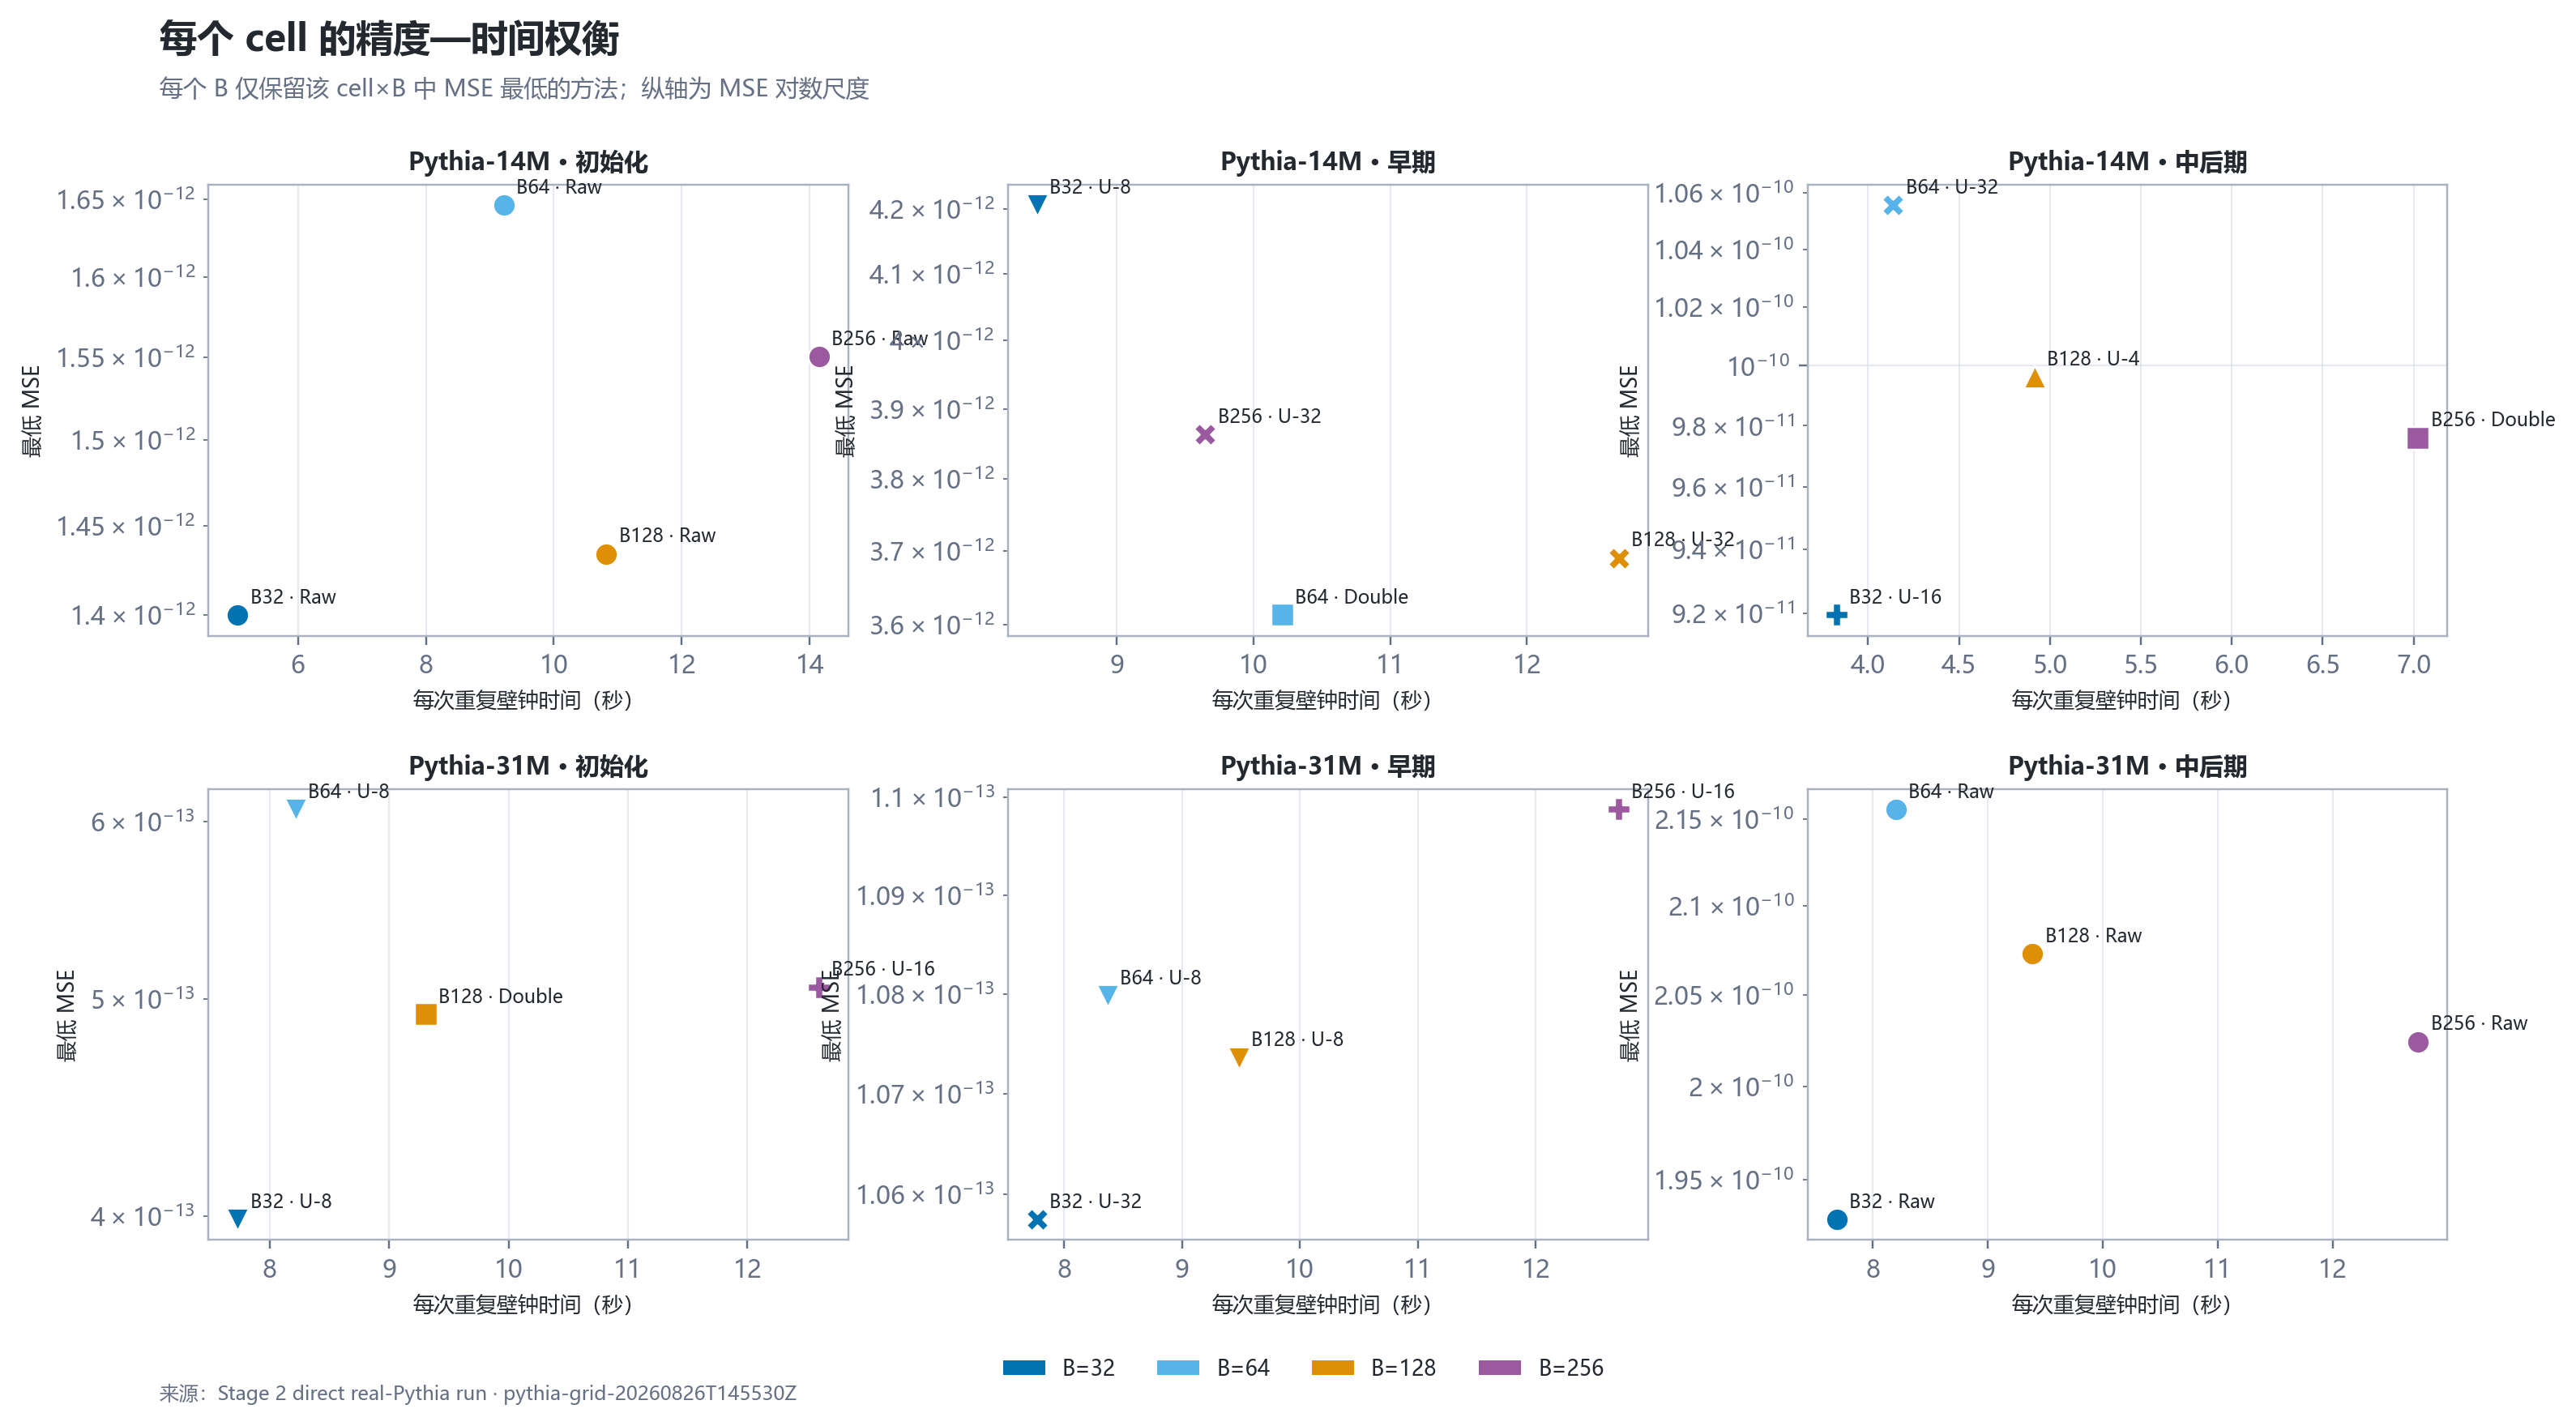
\includegraphics[width=0.96\textwidth]{fig12-accuracy-cost.png}
  \caption{逐 cell 的精度--时间散点。每个 $B$ 标注该 cell$\times B$ 中 MSE 最低的方法。}
  \label{fig:pareto}
\end{figure}

\FloatBarrier

\section{后续实验的估计器选择}

\subsection{默认与阶段化建议}

\begin{center}
\begin{tabularx}{0.98\textwidth}{>{\bfseries}p{2.6cm}p{2.7cm}p{2.5cm}X}
  \toprule
  使用情境 & 主估计器 & 样本预算 & 配套对照与理由 \\
  \midrule
  跨模型、跨阶段统一默认 & \best{U-32} & \best{$B=32$} & 平均 MSE 排名最好；相对 Raw 的几何平均 MSE 低 7.59\%；成本最低档 \\
  初始化阶段 & \best{U-8} & $B=32$ & 同时保留 Raw；U-8 跨两个模型的平均排名最好，Raw 在部分初始化 cell 直接胜出 \\
  训练早期 & \best{U-32} & $B=32$ & Pythia-14M 若追求该 cell 最低观测 MSE，可使用 Double、$B=64$ \\
  中后期 & \best{U-16} 或 U-32 & $B=32$ & 保留 Raw；U-16/U-32 跨场景稳健，Raw 在 Pythia-31M 中后期胜出 \\
  最小双方法方案 & U-32 & $B=32$ & 配 Raw；一条稳健主线加一条高异质性基线 \\
  代数核验 & Double 或 U-2 & 任一 & 两者等价，仅保留一个输出；另一项用于实现不变量检查 \\
  \bottomrule
\end{tabularx}
\end{center}

若后续实验允许记录三种方法，推荐 \method{Raw}+\method{U-16}+
\method{U-32}；初始化专项可将 \method{U-16} 替换为 \method{U-8}。
\method{U-4} 在 24 个场景中仅 1 次排名第一，且平均排名弱于更高 $M$
的 U 估计器；除消融研究外，不建议将其列为主结果。

\subsection{逐 cell 的观测精度}

\begin{center}
\begin{tabular}{llrrrr}
  \toprule
  模型--阶段 & 方法 & $B$ & MSE & MAE & Pearson \\
  \midrule
  14M--初始化 & Raw & 32 & $1.40\times10^{-12}$ & $5.88\times10^{-8}$ & 0.9870 \\
  14M--早期 & Double & 64 & $3.61\times10^{-12}$ & $1.30\times10^{-7}$ & 0.9445 \\
  14M--中后期 & U-16 & 32 & $9.19\times10^{-11}$ & $1.85\times10^{-7}$ & 0.8232 \\
  31M--初始化 & U-8 & 32 & $3.99\times10^{-13}$ & $4.84\times10^{-8}$ & 0.9930 \\
  31M--早期 & U-32 & 32 & $1.06\times10^{-13}$ & $3.20\times10^{-8}$ & 0.8282 \\
  31M--中后期 & Raw & 32 & $1.93\times10^{-10}$ & $2.63\times10^{-7}$ & 0.8982 \\
  \bottomrule
\end{tabular}
\end{center}

以上六个选中配置的 MSE 范围为 $1.06\times10^{-13}$ 至
$1.93\times10^{-10}$，MAE 为 $3.20\times10^{-8}$ 至
$2.63\times10^{-7}$，Pearson 为 0.823 至 0.993。不同 cell 的目标向量
尺度不同，因此这些绝对误差主要用于同一 cell 内方法比较，不宜直接用来
排列训练阶段本身的“难度”。

\section{数据边界与使用说明}

本报告的目的，是把已得到的数据转化为后续实验可执行的估计器选择。使用
这些结论时需要保留以下数据事实：

\begin{itemize}
  \item 结果覆盖两个小型 Pythia 规模和三个训练阶段；跨更大模型时，应首先
    复用 U-32、$B=32$ 默认，并同时保留 Raw 对照。
  \item profiler 在一次 repetition 中联合计算全部估计器，不能据此声称
    某个估计器单独快多少；现有时间结论针对 $B$ 的总体运行成本。
  \item Pythia-31M 中后期 $B=64$ 的候选精度来自 $n=18$ 的续跑汇总；
    其余汇总为 $n=64$。
  \item Double 与 U-2 不构成两个独立证据流；它们的数值一致性应被解释为
    实现不变量，而不是两次独立复现。
\end{itemize}

\section{可复现入口与数据身份}

所有图表和派生 CSV 均由同目录下的 \sourceid{analysis.py} 生成。运行入口：

\begin{verbatim}
python analysis.py --input-root <pythia-grid-20260826T145530Z> \
  --output-root <presentation/Stage 2>
\end{verbatim}

关键身份如下：

\begin{longtable}{>{\bfseries}p{4.3cm}p{10.2cm}}
  \toprule
  字段 & 值 \\
  \midrule
  Run ID & \sourceid{pythia-grid-20260826T145530Z} \\
  Main sweep artifact & \nolinkurl{ff84d8032113da703753282ba1ebdfe9b08bfbb7f36818988870d252ed2b4d4e} \\
  Profiler artifact & \nolinkurl{f33160b33c7a2b3b5afd275243d05e5fb4a48b24d42c3b5ac58e1d14e1174879} \\
  Delivery hash & \nolinkurl{730bf865d2b4eaf60f32cce309560db954a54bbfff4a1cbb69d79383b8c6d78f} \\
  Analysis payload & \nolinkurl{44da7d9fecde8847bc88661db2fd9310928e46ba4d7a851b4ff115a43b567325} \\
  \bottomrule
\end{longtable}

机器可读结果随报告一并交付：
\begin{itemize}
  \item 汇总、来源哈希与逐 cell 推荐：\sourceid{data/analysis-summary.json}；
  \item 完整派生表：\sourceid{data/*.csv}。
\end{itemize}

\section{结论}

Stage 2 数据已经足以给后续实验指定一个明确而不过度简化的选择策略：

\begin{enumerate}
  \item 统一默认使用 \key{U-32、$B=32$}；
  \item 初始化阶段检查 \method{U-8}+\method{Raw}；
  \item 早期阶段优先 \method{U-32}，Pythia-14M 特化点为
    \method{Double}、$B=64$；
  \item 中后期使用 \method{U-16}/\method{U-32}，并保留 Raw；
  \item 不同时保留 Double 与 U-2 作为独立实验分支。
\end{enumerate}

这套选择同时利用了逐 cell 最优结果、跨场景平均排名、偏差--方差位置以及
样本预算的时间成本。最核心的发现不是“某个估计器永远获胜”，而是：
\textbf{U-32 提供最稳健的跨场景默认，Raw 提供不可替代的阶段敏感性对照，
$B=32$ 提供当前数据下最好的精度--成本起点。}

\begin{thebibliography}{9}
\bibitem{hoeffding1948}
W. Hoeffding.
\newblock A Class of Statistics with Asymptotically Normal Distribution.
\newblock \emph{The Annals of Mathematical Statistics}, 19(3), 1948.

\bibitem{biderman2023}
S. Biderman et al.
\newblock Pythia: A Suite for Analyzing Large Language Models Across Training and Scaling.
\newblock \emph{Proceedings of ICML}, 2023.

\bibitem{molchanov2019}
P. Molchanov et al.
\newblock Importance Estimation for Neural Network Pruning.
\newblock \emph{Proceedings of CVPR}, 2019.

\bibitem{stage2data}
Parameter Importance Project.
\newblock Stage 2 direct real-Pythia run: \sourceid{pythia-grid-20260826T145530Z}.
\newblock Internal experiment artifact, 2026.
\end{thebibliography}

\end{document}
